%DOCUMENT CLASS
\documentclass[12pt]{article}

%PACKAGES
\usepackage{amsmath}
\usepackage{amssymb}
\usepackage{amsthm}
\usepackage{array}
\usepackage{comment}
\usepackage{enumerate}
\usepackage{enumitem}
\usepackage[margin=0.5in]{geometry}
\usepackage{mathtools}
\usepackage{tikz}
	\usetikzlibrary{decorations.pathreplacing}
	\usetikzlibrary{through,calc,arrows,intersections,patterns,automata}
	%NEW COMMAND
	\tikzset{
		ncbar angle/.initial=90,
		ncbar/.style={
		to path=(\tikztostart)
		-- ($(\tikztostart)!#1!\pgfkeysvalueof{/tikz/ncbar angle}:(\tikztotarget)$)
		-- ($(\tikztotarget)!($(\tikztostart)!#1!\pgfkeysvalueof{/tikz/ncbar angle}:(\tikztotarget)$)!\pgfkeysvalueof{/tikz/ncbar angle}:
			(\tikztostart)$)
		-- (\tikztotarget)
		},
		ncbar/.default=0.5cm,
		}
	\tikzset{square left brace/.style={ncbar=0.25cm}}
	\tikzset{square right brace/.style={ncbar=-0.25cm}}

%CUSTOM COMMANDS
\newcolumntype{x}[1]{>{\centering\hspace{0pt}}p{#1}}		%Manual-Sized Center Columns
\newcommand{\tn}{\tabularnewline}					 	%Custom New-Line Command

%CUSTOM SETTINGS
\setlength{\parindent}{0pt}							%New Paragraph Indent = 0
\setlist{itemsep = 6pt}						    		%Expands Space Between Items

%FRONT MATTER

\title{Math Camp 2020 - Linear Algebra\footnote{These lecture notes are drawn principally from \emph{Linear Algebra and its Applications}, 4th ed., by David C. Lay and \emph{Fundamental Methods of Mathematical Economics}, 4th ed., by Alpha C. Chiang and Kevin Wainwright. The material posted on this website is for personal use only and
		is not intended for reproduction, distribution, or citation.}
}
\date{\normalsize \today}
\author{\normalsize Created by James Banovetz \\ { \normalsize Modified by Woongchan Jeon } \\[12pt] \normalsize Department of Economics, UC Santa Barbara}

%Begin Document
\begin{document}

\maketitle

\begin{enumerate}

%%%%%%%%%
%LAY 1.1%
%%%%%%%%%
\item\textbf{Systems of Linear Equations and Matrices}
	\begin{enumerate}
	\item\underline{\smash{Definition}}.
		A \textbf{linear equation} in the variables $x_1,x_2,\cdots,x_n$ is an equation that can be written in the form
			\[a_1x_1+a_2x_2+\dots+a_nx_n = b\]
		where $b$ and the coefficients $a_1,\dots,a_n$ are real or complex numbers. A \textbf{system of linear equations} is a collection of one or more linear equations involving the same variables.

	\item\underline{\smash{Example}}.
		Consider the following system of linear equations:
			\begin{align*}
				x_1 - 2x_2 + x_3 & = 0 \\
				2x_2 - 8x_3 & = 8 \\
				-4x_1+5x_2+9x_3 & = -9
			\end{align*}

	\item\underline{\smash{Defintion}}.
		The compact rectangular array containing the coefficients of each variable aligned in columns
		is called the \textbf{coefficient matrix}.

	\item\underline{\smash{Example}}.
		From the system of linear equations above, the coefficient matrix is
			\[\begin{bmatrix}
				1	&-2	&1	\\
				0	&2	&-8	\\
				-4	&5	&9
			\end{bmatrix}\]

	\item\underline{\smash{Definition}}.
		The coefficient matrix, concatenated with a column consisting of the right-hand-side constants
		is called the \textbf{augmented matrix}.
	
	\item\underline{\smash{Example}}.
		From the system of linear equations above, the augmented matrix is
			\[\left[\begin{array}{c c c | c}
				1	&-2	&1	&0	\\
				0	&2	&-8	&8	\\
				-4	&5	&9	&-9
			\end{array}\right]\]

\vspace{5mm}

	\item\underline{\smash{Definition}}.
		The \textbf{size} of a matrix tells how many rows and columns it has.
		An $m\times n$ matrix has $m$ rows and $n$ columns:
			\[\begin{bmatrix}
				a_{11}	& a_{12}	& a_{13}	& \dots	& a_{1n}	\\
				a_{21}	& a_{22}	& a_{23}	& \dots	& a_{2n}	\\
				a_{31}	& a_{32}	& a_{33}	& \dots	& a_{3n}	\\
				\vdots	& \vdots	& \vdots	& \ddots	& \vdots	\\
				a_{m1}	& a_{m2}	& a_{m3}	& \dots	& a_{mn}
			\end{bmatrix}\]

	\item\underline{Definition}. The \textbf{element} $a_{ij}$ is the value in row $i$, column $j$

	\item\underline{Definition}.
		To solve the system of equations, the three basic operations are known as \textbf{elementary row operations}.
		These operations consist of:
		\begin{itemize}
		\item Scaling - Multiply all entries in a row by a non-zero constant
		\item Replacement - Replace one row by the sum of itself and the multiple of another row
		\item Interchange - Interchange any two rows
		\end{itemize}

	\item\underline{\smash{Example}}.
		Consider the augmented matrix from our system above:
			\begin{align*}
				\left[\begin{array}{c c c | c}
				1	&-2	&1	&0	\\
				0	&2	&-8	&8	\\
				-4	&5	&9	&-9
				\end{array}\right]
			&\hspace{20pt}\rightarrow\text{Multiplying $R_2$ by 1/2:}\rightarrow
				& \left[\begin{array}{c c c | c}
				1	&-2	&1	&0	\\
				0	&1	&-4	&4	\\
				-4	&5	&9	&-9
				\end{array}\right]\\[10pt]
			\intertext{Replacing $R_3$ with $R_3+4R_1$:}
				\left[\begin{array}{c c c | c}
				1	&-2	&1	&0	\\
				0	&1	&-4	&4	\\
				0	&-3	&13	&-9
				\end{array}\right]
			&\hspace{20pt}\rightarrow\text{Replacing $R_3$ with $R_3+3R_2$:}\rightarrow
				& \left[\begin{array}{c c c | c}
				1	&-2	&1	&0	\\
				0	&1	&-4	&4	\\
				0	&0	&1	&3
				\end{array}\right]\\[10pt]
			\intertext{Replacing $R_2$ with $R_2+4R_3$:}
				\left[\begin{array}{c c c | c}
				1	&-2	&1	&0	\\
				0	&1	&0	&16	\\
				0	&0	&1	&3
				\end{array}\right]
			&\hspace{20pt}\rightarrow\text{Replacing $R_1$ with $R_1-R_3$:}\rightarrow
				& \left[\begin{array}{c c c | c}
				1	&-2	&0	&-3	\\
				0	&1	&0	&16	\\
				0	&0	&1	&3
				\end{array}\right]\\[10pt]
			\intertext{Replacing $R_1$ with $R_1+2R_2$:}
				\left[\begin{array}{c c c | c}
				1	&0	&0	&29	\\
				0	&1	&0	&16	\\
				0	&0	&1	&3
				\end{array}\right]
			&\hspace{20pt}\rightarrow\text{The simplified system:}\rightarrow&\begin{array}{c c c c c}
				x_1	&	&	&=	&29	\\
					&x_2	&	&=	&16	\\
					&	&x_3	&=	&3
				\end{array}
			\end{align*}

	\item\underline{\smash{Aside}}.
		This matrix is now in what we call \textbf{reduced row echelon form}. Don't worry about the terminology, however,
		what's important is the row operations, which may come in handy a few times throughout the year. Also note
		that not all linear systems have unique solutions; it is possible to have a unique solution, infinite solutions,
		or no solutions.
	\end{enumerate}

\newpage

%%%%%%%%%
%LAY 1.3%
%%%%%%%%%
\item\textbf{Vectors and Vector Equations}
	\begin{enumerate}
	\item\underline{Definition}: A \textbf{column vector} is a $n\times 1$ matrix: 
			\[\begin{bmatrix}
				a_{11} \\
				\vdots \\
				a_{n1}
			\end{bmatrix}
			\quad\text{or}\quad
			\begin{bmatrix}
				a_{1} \\
				\vdots \\
				a_{n}
			\end{bmatrix}\]
		While a \textbf{row vector} is a $1\times m$ matrix:
			\[\begin{bmatrix}
				a_{11} &
				\cdots &
				a_{1m}
			\end{bmatrix}
			\quad\text{or}\quad
			\begin{bmatrix}
				a_{1} &
				\cdots &
				a_{m}
			\end{bmatrix}\]

	\item\underline{\smash{Example}}.
		Consider the $2\times 1$ vectors $\mathbf{u}=\begin{bmatrix}2 \\ 1\end{bmatrix}$ and $\mathbf{v}=\begin{bmatrix}1 \\ 2\end{bmatrix}$.
		These vectors ``live" in $\mathbb{R}^2$ (the set of ordered pairs of real numbers). Geometrically, we can interpret $\mathbb{R}^2$
		as a 2-dimensional plane and vectors as points on the plane: 
		\begin{center}
			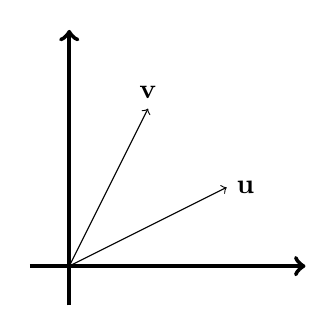
\begin{tikzpicture}
				%AXES
				\draw[ultra thick,->](-.5,0)--(3,0);
				\draw[ultra thick,->](0,-.5)--(0,3);
				%VECTORS
				\draw[->](0,0)--(2,1)node[right]{$\mathbf{u}$};
				\draw[->](0,0)--(1,2)node[above]{$\mathbf{v}$};
			\end{tikzpicture}
		\end{center}
	
	\item\underline{\smash{Aside}}.
		A vector is a quantity that has magnitude and direction. A directed line segment is a line segment that has both a starting and an end point, so it has a direction.

	\item\underline{\smash{Aside}}.
		Note that analagous interpretations apply to higher-dimensional spaces (e.g., $\mathbb{R}^3$, $\mathbb{R}^4$, etc.), but
		it's visually much easier to picture things in 2-dimensions.

	\item\underline{\smash{Definition}}.
		Two vectors in $\mathbb{R}^n$ are \textbf{equal} if and only if their corresponding elements are equal.

	\item\underline{\smash{Example}}.
		Our vectors from above, $\mathbf{u}=\begin{bmatrix}2 \\ 1\end{bmatrix}$ and $\mathbf{v}=\begin{bmatrix}1 \\ 2\end{bmatrix}$,
		are \emph{not} equal.

	\item\underline{\smash{Definition}}.
		Given two vectors $\mathbf{u}$ and $\mathbf{v}$, their \textbf{sum} is the vector $\mathbf{u}+\mathbf{v}$, obtained
		by adding the corresponding elements.

	\item\underline{\smash{Example}}.
		Consider the vectors $\mathbf{u}=\begin{bmatrix}2 \\ 1\end{bmatrix}$ and $\mathbf{v}=\begin{bmatrix}1 \\ 2\end{bmatrix}$.
			\[\mathbf{u}+\mathbf{v}=\begin{bmatrix}2 \\ 1\end{bmatrix}+\begin{bmatrix}1 \\ 2\end{bmatrix}=
				\begin{bmatrix} 3 \\ 3 \end{bmatrix}\]
	
	\item\underline{\smash{Definition}}.
		Given a vector $\mathbf{u}$ and a real number $c$, the \textbf{scalar multiple} of $\mathbf{u}$ by $c$ is the vector	obtained by multiplying each element in $\mathbf{u}$ by $c$.

	\item\underline{\smash{Example}}.
		Consider the vector $\mathbf{u}=\begin{bmatrix}2 \\ 1\end{bmatrix}$ and the scalar $c=3$. Then:
			\[c\mathbf{u}=3\begin{bmatrix}2 \\ 1 \end{bmatrix}=\begin{bmatrix}6\\3\end{bmatrix}\]
	
	\item\underline{\smash{Definition}}.
	Two vectors $\mathbf{u}$ and $\mathbf{v}$ in $\mathbb{R}^n$ are parallel if and only if there exists a real number $c \in \mathbb{R}\setminus \{0\}$ such that 
		\[ \mathbf{u} = c \mathbf{v} \]

	\item\underline{\smash{Definition}}.
		Given vectors $\mathbf{{v}}_1,\mathbf{{v}}_2,\cdots,\mathbf{{v}}_k$ and scalars $c_1,c_2,\cdots,c_k$, the vector $\mathbf{{y}}$ defined by
			\[ \mathbf{{y}}=c_1\mathbf{{v}}_1+\cdots+c_k\mathbf{{v}}_k \]
		is called a \textbf{linear combination} of $\mathbf{{v}}_1,\cdots,\mathbf{{v}}_k$ with weights $c_1,\cdots,c_k$.

	\item\underline{\smash{Definition}}. %From Lay THM 1.7
		A set of vectors $\mathbf{{v}}_1,\cdots,\mathbf{{v}}_k \in \mathbb{R}^n$ is \textbf{linearly dependent} if and only if at least one of the vectors can be written as a linear combination of the others. If no vector is a linear combination of the others, the set of fectors are \textbf{linearly independent}.

		\textbf{Remark} A set of vectors $\mathbf{{v}}_1,\cdots,\mathbf{{v}}_k \in \mathbb{R}^n$ is \textbf{linearly independent} if and only if the vector equation 
		\[ c_1 \mathbf{{v}}_1 + c_2 \mathbf{{v}}_2 + \cdots + c_k \mathbf{{v}}_k = \mathbf{0}_n \]
		has only the trivial solution. 
		
	\item\underline{\smash{Aside}}. Let us assume that $\mathbf{{v}}_1,\cdots,\mathbf{{v}}_k \in \mathbb{R}^n$ is linearly dependent. WLOG, there exists $i \in \{1, \cdots, k\}$ such that $c_i \neq 0$. Then 
		\begin{align*}
			c_i \mathbf{v}_i + \sum_{j=1, \ j \neq i}^k c_j \mathbf{v}_j = \mathbf{0}_n  \hspace{5mm} \mbox{and} \hspace{5mm}	\mathbf{v}_i = - \sum_{j=1, \ j \neq i}^k \frac{c_j}{c_i} \mathbf{v}_j
		\end{align*}
		
	\item\underline{\smash{Example}}.
		Consider the vectors:
		\[\mathbf{{v}}_1=\begin{bmatrix}1\\2\\3\end{bmatrix},\quad\mathbf{{v}}_2=\begin{bmatrix}4\\5\\6\end{bmatrix},
			\quad\mathbf{{v}}_3=\begin{bmatrix}2\\1\\0\end{bmatrix}\]
		By inspection, $\mathbf{{v}}_3=-2\mathbf{{v}}_1+\mathbf{{v}}_2$, so the vectors are linearly dependent.

	\item\underline{\smash{Definition}}.
		If $\mathbf{{v}}_1,\cdots,\mathbf{{v}}_k\in\mathbb{R}^n$, then the set of all linear combinations of $\mathbf{{v}}_1,\cdots,\mathbf{{v}}_k$ is called \textbf{span} of $\mathbf{{v}}_1,\cdots,\mathbf{{v}}_k$. That is, the span is collection of all vectors that can be
		written in the form 
			\[ \Big\{ \mathbf{{w}} \in \mathbb{R}^n \ : \ \mathbf{{w}} = c_1\mathbf{{v}}_1+c_2\mathbf{{v}}_2+\cdots+c_k\mathbf{{v}}_k \ \text{  for any  } \ [ c_1 \ \cdots \ c_k ]' \in \mathbb{R}^k \Big\}\]
		
	\item\underline{\smash{Definition}}.
		$\mathbf{{v}}_1,\cdots,\mathbf{{v}}_k\in\mathbb{R}^n$ spans $\mathbb{W}$ if given any $\mathbf{{w}} \in \mathbb{W}$,
		\[ \exists \ [c_1 \ \cdots \ c_k]' \in \mathbb{R}^k \ \ni \ \mathbf{{w}} = \sum_{i=1}^k c_i \mathbf{{v}}_i \]
		
	\item\underline{\smash{Definition}}.
	$\mathbf{{v}}_1,\cdots,\mathbf{{v}}_k\in \mathbb{W} \subset \mathbb{R}^n$ forms a basis of $\mathbb{W}$ if 
		\begin{enumerate}
			\item $\mathbf{{v}}_1,\cdots,\mathbf{{v}}_k$ spans $\mathbb{W}$, and 
			\item $\mathbf{{v}}_1,\cdots,\mathbf{{v}}_k$ are linearly independent. 
		\end{enumerate} 
		
	\item\underline{\smash{Example}}.
	Consider the vectors $\begin{bmatrix}1 \\ 0\end{bmatrix}$ and $\begin{bmatrix}0 \\ -2\end{bmatrix}$. These vectors span
	$\mathbb{R}^2$; any vector in $\mathbb{R}^2$ can be written as a linear combination of these two vectors.
	
\newpage
	
	\end{enumerate}

%%%%%%%%%
%LAY 1.4%
%%%%%%%%%

\item\textbf{The Matrix Equation}
	\begin{enumerate}
	\item\underline{\smash{Definition}}.
		If $\mathcal{A}$ is an $m\times n$ matrix with columns $\mathbf{{a}}_1,\cdots,\mathbf{{a}}_n \in \mathbb{R}^m$, and if $\mathbf{{x}}\in\mathbb{R}^n$,
		then the \textbf{product} of $\mathcal{A}$ and $\mathbf{{x}}$, denoted $\mathcal{A}\mathbf{{x}}$, is the linear combination of the columns of $\mathcal{A}$ using the corresponding entries in $\mathbf{x}$ as weights
			\[ \mathcal{A}\mathbf{{x}}=\begin{bmatrix} & & \\  & & \\ \mathbf{{a}}_1&\cdots&\mathbf{{a}}_n \\  & & \\  & & \end{bmatrix}
				\begin{bmatrix}x_1 \\ \vdots \\ x_n\end{bmatrix}
				=x_1\mathbf{{a}}_1+\cdots+x_n\mathbf{{a}}_n \hspace{20mm} \text{\bf (Column Expansion)} \]
		and the equation $\mathcal{A}\mathbf{{x}}=\mathbf{{b}}$ is called a \textbf{matrix equation}.

	\item\underline{\smash{Theorem}} (Lay THM 1.3).
		If $\mathcal{A}$ is a $m\times n$ matrix with columns $\mathbf{a}_1,\dots,\mathbf{a}_n \in \mathbb{R}^m$ and if $\mathbf{b}\in\mathbb{R}^m$, then the
		matrix equation $\mathcal{A}\mathbf{x}=\mathbf{b}$ has the same solution set as the linear equations whose augmented matrix
		is \[\left[\begin{array}{c c c | c}\mathbf{a}_1&\cdots&\mathbf{a}_n&\mathbf{b}\end{array}\right]\]

	\item\underline{\smash{Example}}.
		Consider our first example, the linear system:
			\begin{align*}
				x_1 - 2x_2 + x_3 & = 0 \\
				2x_2 - 8x_3 & = 8 \\
				-4x_1+5x_2+9x_3 & = -9
			\end{align*}
		Let $\mathcal{A}$ be the coefficient matrix:
			\[\mathcal{A} = \begin{bmatrix}
				1	&-2	&1	\\
				0	&2	&-8	\\
				-4	&5	&9
			\end{bmatrix}\]
		Then we can rewrite the linear system as a matrix equation $\mathcal{A}\mathbf{x}=\mathbf{b}$:
			\[\begin{bmatrix}
				1	&-2	&1	\\
				0	&2	&-8	\\
				-4	&5	&9
			\end{bmatrix}
			\begin{bmatrix} x_1 \\ x_2 \\ x_3\end{bmatrix}
			=
			\begin{bmatrix}
			0 \\ 8 \\ -9
			\end{bmatrix}\]
	
	\item\underline{\smash{Aside}}.
		We won't worry too much about the matrix equation right now, but note that this is reminiscent of our matrix representation of OLS. We'll work with this type of equation quite a bit during the first year.
		\begin{align*}
			y_i &= x_{i1} \beta_1 + x_{i2}\beta_2 + \cdots + x_{ik-1} \beta_{k-1} + \beta_k + u_i \hspace{5mm} &\forall \ i=1, \cdots, n \\ 
				& = \mathbf{x}_i\hspace{0mm}^T  \boldsymbol{\beta} + u_i &\forall \ i=1, \cdots, n
		\end{align*}
		\[ \mathbf{y} = \mathcal{X} \boldsymbol{\beta} + \mathbf{u}  \]
		
	\end{enumerate}



%%%%%%%%%
%LAY 2.1%
%%%%%%%%%
\item\textbf{Matrix Operations}
	\begin{enumerate}
	\item\underline{\smash{Definition}}. Let $\mathcal{A}$ and $\mathcal{B}$ be $m\times n$ matrices. Let $a_{ij}$ and $b_{ij}$ denote the elements in the $i$th
		row and $j$th column of the matrices $\mathcal{A}$ and $\mathcal{B}$, respectively. Then $\mathcal{A}$ and $\mathcal{B}$ are \textbf{equal},
		denoted $\mathcal{A}=\mathcal{B}$, if and only if $a_{ij}=b_{ij}$ for all $i$ and all $j$.

	\item\underline{\smash{Aside}}.
		Note that this is simply an extension of our definition for vector equality; indeed, we could define matrix equality in
		terms of vector equality, i.e., two matrices are equal if and only if their corresponding vectors are equal.

	\item\underline{\smash{Definition}}.
		If $\mathcal{A}$ and $\mathcal{B}$ are both $m\times n$ matrices, then the \textbf{sum} $\mathcal{A}+\mathcal{B}$ is the $m\times n$ matrix whose elements are the sums
		of the corresponding elements from $\mathcal{A}$ and $\mathcal{B}$. The \textbf{difference} $\mathcal{A}-\mathcal{B}$ is the $m\times n$ matrix whose elements are the differences of the corresponding elements of $\mathcal{A}$ and $\mathcal{B}$.
			\[\mathcal{A}+\mathcal{B} = \begin{bmatrix}    a_{11} 		&a_{12}		&\cdots 		&a_{1n}	\\
														a_{21} 		 &a_{22}		&\cdots 		&a_{2n}  \\
														\vdots		&\vdots	 	&\ddots	  &\vdots	\\ 
														a_{m1} 		&a_{m2} 	&\dots 	  &a_{mn}\end{bmatrix}
					+\begin{bmatrix}    b_{11} 		&b_{12}		&\cdots 		&b_{1n}	\\
													b_{21} 		&b_{22}		&\cdots 		&b_{2n}  \\
													\vdots		&\vdots	 	&\ddots	  &\vdots	\\ 
													b_{m1} 		&b_{m2} 	&\cdots 	  &b_{mn}\end{bmatrix}
					=\begin{bmatrix}    a_{11}+b_{11} 			&a_{12}+b_{12}		&\cdots 	  &a_{1n}+b_{1n}	\\
													a_{21}+b_{21} 			&a_{22}+b_{22}	&\dots 		&a_{2n}+b_{2n}  \\
													\vdots						&\vdots	 				&\ddots	  &\vdots	\\ 
													a_{m1}+b_{m1} 		&a_{m2}+b_{m2}	&\cdots 	  &a_{mn}+b_{mn} \end{bmatrix}\]

	\item\underline{\smash{Definition}}.
		If $k$ is a scalar and $A$ is a matrix, then the \textbf{scalar multiple} $k\mathcal{A}$ is the matrix whose elements are $k$ times the corresponding elements in $\mathcal{A}$.
				\[k\mathcal{A}=\begin{bmatrix}
						ka_{11} 	 & ka_{12} 	 & \cdots  	& ka_{1n}\\
						ka_{21} 	& ka_{22} 	& \cdots    & ka_{2n}\\
						\vdots 		& \vdots 	 & \ddots  & \vdots  \\ 
						ka_{m1}    & ka_{m2}  & \cdots    & ka_{mn}
				\end{bmatrix}\]
	
	\item\underline{\smash{Definition}}.
		If $\mathcal{A}$ is a $m\times n$ matrix and $\mathcal{B}$ is a $n\times k$ matrix with columns $\mathbf{b}_1,\cdots,\mathbf{b}_k$, then the \textbf{product} $\mathcal{AB}$ is the $m\times k$ matrix whose columns are  $\mathcal{A}\mathbf{b}_1,\cdots,\mathcal{A}\mathbf{b}_k$. Note that the number of columns of $\mathcal{A}$ must match the number of rows in $\mathcal{B}$ for the matrices to be conformable.

	\item\underline{\smash{Example}}.
		Suppose we have two matrices: $\mathcal{A}_{1\times 2}$ and $\mathcal{B}_{2\times 3}$. Then $\mathcal{AB}$ is permissible, but $\mathcal{BA}$ is not.
		If we have $\mathcal{A}_{1\times 2}\mathcal{B}_{2\times 3}=\mathcal{C}_{1\times 3}$, then
		\begin{itemize}
		\item For $c_{11}$: $c_{11}=a_{11}b_{11}+a_{12}b_{21}$
			\begin{center}
				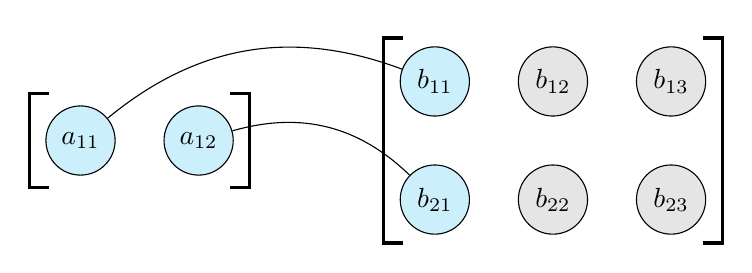
\begin{tikzpicture}[auto,node distance=1.5cm]
					\tikzstyle{every state}=[fill=cyan!20]
					%NODES for A Matrix
					\node[state](a11){$a_{11}$};
					\node[state](a12)[right of = a11]{$a_{12}$};
					%NODES for B Matrix
					\node[state](b11)[right of = a12, xshift=15mm, yshift=7.5mm]{$b_{11}$};
					\node[state](b21)[below of = b11]{$b_{21}$};
					\node[state,fill=gray!20](b12)[right of = b11]{$b_{12}$};
					\node[state,fill=gray!20](b22)[below of = b12]{$b_{22}$};
					\node[state,fill=gray!20](b13)[right of = b12]{$b_{13}$};
					\node[state,fill=gray!20](b23)[below of = b13]{$b_{23}$};
					%PATHS
					\path	(a11) edge [bend left] node {} (b11)
					(a12) edge [bend left] node {} (b21);
					%BRACKETS
					\draw [very thick] (-.4,-.6) to [square left brace ] (-.4,.6);
					\draw [very thick] (1.9,-.6) to [square right brace ] (1.9,.6);
					\draw [very thick] (4.1,-1.3) to [square left brace] (4.1,1.3);
					\draw [very thick] (7.9,-1.3) to [square right brace] (7.9,1.3);
				\end{tikzpicture}
			\end{center}
		\item For $c_{12}$: $c_{12}=a_{11}b_{12}+a_{12}b_{22}$
			\begin{center}
				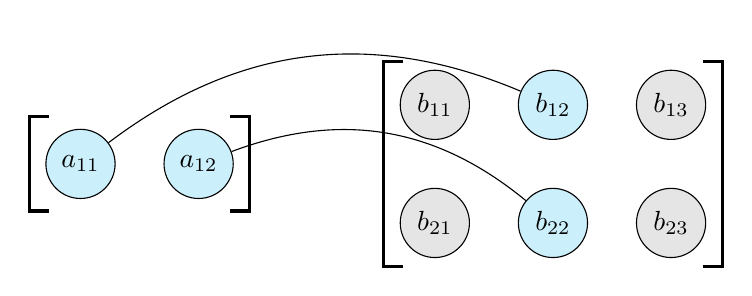
\begin{tikzpicture}[auto,node distance=1.5cm]
					\tikzstyle{every state}=[fill=cyan!20]
					%NODES for A Matrix
					\node[state](a11){$a_{11}$};
					\node[state](a12)[right of = a11]{$a_{12}$};
					%NODES for B Matrix
					\node[state,fill=gray!20](b11)[right of = a12, xshift=15mm, yshift=7.5mm]{$b_{11}$};
					\node[state,fill=gray!20](b21)[below of = b11]{$b_{21}$};
					\node[state](b12)[right of = b11]{$b_{12}$};
					\node[state](b22)[below of = b12]{$b_{22}$};
					\node[state,fill=gray!20](b13)[right of = b12]{$b_{13}$};
					\node[state,fill=gray!20](b23)[below of = b13]{$b_{23}$};
					%PATHS
					\path	(a11) edge [bend left] node {} (b12)
					(a12) edge [bend left] node {} (b22);
					%BRACKETS
					\draw [very thick] (-.4,-.6) to [square left brace ] (-.4,.6);
					\draw [very thick] (1.9,-.6) to [square right brace ] (1.9,.6);
					\draw [very thick] (4.1,-1.3) to [square left brace] (4.1,1.3);
					\draw [very thick] (7.9,-1.3) to [square right brace] (7.9,1.3);
				\end{tikzpicture}
			\end{center}
		\end{itemize}

	%%%%%%%%%%%%
	%CHIANG 4.5%
	%%%%%%%%%%%%
	\item\underline{\smash{Aside}.}
		There are a few special matrices with which you should be familiar. For example:
		\begin{enumerate}
		\item The Identity Matrix (a diagonal matrix of ones)
				\[ \mathcal{I}_n = \begin{bmatrix}
								1			&0			& \cdots 	&0	\\
								0			&1			& \cdots 	&0		\\
								\vdots	&\vdots & \ddots   & \vdots \\
								0 			& 0 	   & \cdots     &1 	
							\end{bmatrix} \]
			Note that for all $n$ by $n$ matrices $\mathcal{A}$:
				\[\mathcal{A}\mathcal{I}_n = \mathcal{I}_n\mathcal{A} = \mathcal{A}\]

		\item The Null Matrix (a matrix of zeros)
				\[\mathbf{0}_{m\times n} = \begin{bmatrix}
								0 & 0 & 0 & \cdots & 0 \\
								0 & 0 & 0 &	\cdots & 0	\\
								\vdots& \vdots& \vdots &\ddots & \vdots \\
								0 & 0 & 0 & \cdots &0	\end{bmatrix}\]
			Note that for all matrices $\mathcal{A}$ and ``conformable" matrices $\mathbf{0}$:
				\begin{align*}
					\mathcal{A} + \mathbf{0}	& = \mathcal{A} 			&\mathbf{0} + \mathcal{A}	& = \mathcal{A} \\
					\mathbf{0}\mathcal{A}		& = \mathbf{0}	&A\mathbf{0}	& = \mathbf{0}
				\end{align*}
		\item Idempotent Matrices (a matrix that is the product of itself)
				\[\mathcal{A}= \mathcal{AA}\]
		\end{enumerate}
	 
	\item\underline{\smash{Theorem}} (Lay THM 2.2)
		Let $\mathcal{A}$ be a $m\times n$ matrix, and let $\mathcal{B}$ and $\mathcal{C}$ have dimensions for which the indicated sums and products are defined. Then
		\begin{align*}
			&\mathcal{A(BC) = (AB)C = ABC}	&\text{(Associative Law)}			\\
			&\mathcal{A(B+C) = AB+AC}		&\text{(Left Distributive Law)}		\\
			&\mathcal{(B+C)A = BA+CA}		&\text{(Right Distributive Law)}	
		\end{align*}

	\item\underline{\smash{Aside}}.
		Note that in matrix algebra, we \emph{do not} have commutativity; that is, $\mathcal{AB\neq BA}$ in general.
		It may be true of specific matrices, but in many cases (as in an example above), the matrices won't
		even be conformable in both orders.

	\item\underline{\smash{Definition}}.
		Given a $m\times n$ matrix $\mathcal{A}$, the \textbf{transpose} of $\mathcal{A}$ is the $n\times m$ matrix, denoted $\mathcal{A}^T$ or $\mathcal{A}'$, whose columns are formed from the corresponding rows of $\mathcal{A}$.

	\item\underline{\smash{Example}}.
		Consider the following matrices:
			\begin{align*}
				\mathcal{A}	& = \begin{bmatrix}3 & 8 & -9 \\ 1 & 0 & 4\end{bmatrix}
				&\mathcal{B} & = \begin{bmatrix}3 & 4 \\ 1 & 7\end{bmatrix} \\[10pt]
				\mathcal{A}^T & = \begin{bmatrix}3 & 1 \\  8 & 0 \\ -9 & 4\end{bmatrix}
					&\mathcal{B}^T &= \begin{bmatrix}3 & 1 \\ 4 & 7\end{bmatrix}
			\end{align*}
	
	\textbf{Remark}
		A property of matrices that occasionally comes in handy is symmetry, when $\mathcal{A = A}^T$. Later on, we'll talk about Hessian matrices, which have this property.

	\item\underline{\smash{Theorem}} (Lay THM 2.3).
		Let $\mathcal{A}$ and $\mathcal{B}$ denote matrices whose sizes are appropriate for the following sums and products.
			\begin{align*}
				(\mathcal{A}^T)^T 	&= \mathcal{A}			\\
				(\mathcal{A+B})^T	&= \mathcal{A}^T + \mathcal{B}^T	\\
				(\mathcal{AB})^T	&= \mathcal{B}^T\mathcal{A}^T
			\end{align*}

\newpage

	%%%%%%%%%%%%
	%CHIANG 5.2%
	%%%%%%%%%%%%
	\item \underline{\smash{Definition}}.
		The \textbf{determinant} of a square matrix $\mathcal{A}$, denoted by $|\mathcal{A}|$ or $\text{det}(\mathcal{A})$, is a uniquely defined scalar associated with the matrix. For matrices of various sizes:
		\begin{enumerate}
		\item $1\times1$ Matrix: $\mathcal{A}=[a]$
			\[|\mathcal{A}|=a\]\\[-20pt]

		\item $2\times 2$ Matrix: $\mathcal{A}=\begin{bmatrix}
									a & b \\ 
									c & d
									\end{bmatrix}$
			\[|\mathcal{A}| = \begin{vmatrix}
						a & b \\ 
						c & d \end{vmatrix}
						=ad-bc\]\\[-20pt]
						
		\item Larger Matrix: Check the appendix
		\end{enumerate}
	
	%%%%%%%%%%%%
	%CHIANG 5.2%
	%%%%%%%%%%%%
	\item\underline{\smash{Theorem}} (CW SEC 5.3).
		\begin{enumerate}
		\item Taking the transpose does not affect the determinant:
			\[|\mathcal{A}|=|\mathcal{A}^T|\]

		\item Scaling a row by $k$ will change the value of the determinant $k$-fold, e.g.:
			\[\begin{vmatrix}
				ka	&kb	\\ 
				c	&d	\end{vmatrix}
			= k \begin{vmatrix}
				a 	&b	\\
				c	&d	\end{vmatrix}\]

		\item Replacement--adding a multiple of a row (or column) to another row (or column)--leaves the determinant unchanged, e.g.:
			\[\begin{vmatrix}
				a	&b		\\
				c+ka	&d+kb	\end{vmatrix}
			=\begin{vmatrix}
				a	&b		\\
				c	&d		\end{vmatrix}\]

		\item Interchanging any two rows (or columns) reverses the sign of the determinant (but does not change the absolute value), e.g.:
			\[\begin{vmatrix}a & b \\ c & d \end{vmatrix} = - \begin{vmatrix} c & d \\ a & b\end{vmatrix}\]
		\end{enumerate}
			
	\item\underline{\smash{Definition}}.
		A matrix $\mathcal{A}$ is \textbf{singular} if and only if
					\[|\mathcal{A}|=0\]
		which occurs only when rows (or columns) are linearly dependent.
	
	\textbf{Remark}
		I'm bringing this to your attention primarily for econometric reasons; perfect-collinearity means that two of your
		explanatory variables are linear combinations of one another. In this case, STATA, R, or whatever program you
		ultimately use to run regressions will fail (as they use matrix algebra to do OLS).
	

	%%%%%%%%%
	%LAY 2.2%
	%%%%%%%%%
	\item\underline{\smash{Definition}}.
		A $n\times n$ matrix is said to be \textbf{invertible} if there is an $n\times n$ matrix $\mathcal{C}$ such that
			\[\mathcal{CA} = \mathcal{I}_n \quad\text{ and }\quad \mathcal{AC} = \mathcal{I}_n\]
		In this case, $\mathcal{C}$ is the \textbf{inverse} of $\mathcal{A}$. In fact, the inverse is unique, so it is typically
		denoted $\mathcal{A}^{-1}$.

\newpage

	\item\underline{\smash{Theorem}} (Lay THM 2.4).
		If $\mathcal{A}$ is a $2\times 2$ matrix
			\[\mathcal{A}=\begin{bmatrix}
				a & b \\ c & d
				\end{bmatrix}\]
		and $ad-bc\neq 0$ (i.e., the determinant is non-zero/the matrix is non-singular), then the inverse is
			given by the formula:
			\[\mathcal{A}^{-1}=\frac{1}{ad-bc}\begin{bmatrix}d & -b \\ -c & a\end{bmatrix}\]
		
		Check the appendix for a larger matrix.
	\item\underline{\smash{Example}}.
		Consider the matrix
			\[\mathcal{A}=\begin{bmatrix}3 & 4 \\ 5 & 6\end{bmatrix}\]
		Since the determinant is $|\mathcal{A}|=(3*6)-(4*5)=-2\neq0$, $\mathcal{A}$ is invertible:
		\begin{align*}
			|\mathcal{A}| & = -2													&\text{(the determinant)}\\
			\mathcal{A}^{-1} & = \frac{1}{-2}\begin{bmatrix}6 & -4 \\ -5 & 3\end{bmatrix}	&\text{(by THM 2.4)}\\
			\mathcal{A}^{-1} & = \begin{bmatrix}-3 & 2 \\ 5/2 & -3/2\end{bmatrix}		&\text{(simplifying)}
		\intertext{Checking to make sure we did everything properly:}
			\mathcal{A}\mathcal{A}^{-1} & = \begin{bmatrix}3 & 4 \\ 5 & 6\end{bmatrix}\begin{bmatrix}-3 & 2 \\ 5/2 & -3/2\end{bmatrix}
					&\text{(multiplying matrices)}\\
			\mathcal{A}\mathcal{A}^{-1}& = \begin{bmatrix} 1 & 0 \\ 0 & 1 \end{bmatrix}
					&\text{(simplifying)}
		\end{align*}

	\item\underline{\smash{Theorem}} (Lay THM 2.6).
		If $\mathcal{A}$ and $\mathcal{B}$ are $n\times n$ invertible matrices, then
		\begin{enumerate}
		\item $\mathcal{A}^{-1}$ is invertible and
				\[(\mathcal{A}^{-1})^{-1}=\mathcal{A}\]
		\item $\mathcal{AB}$ is invertible and
				\[(\mathcal{AB})^{-1} = \mathcal{B}^{-1}\mathcal{A}^{-1}\]
		\item $\mathcal{A}^T$ is invertible and
				\[(\mathcal{A}^T)^{-1}=(\mathcal{A}^{-1})^T\]
		\end{enumerate}
	
	\item\underline{\smash{Example}}. Given a $n \times k$ matrix $\mathcal{X}$ where $n>k$, assume that $\mathcal{X}^T \mathcal{X}$ is invertible. 
		\begin{align*}
			\Big( \mathcal{X} \big(\mathcal{X}^T \mathcal{X} \big)^{-1} \mathcal{X}^T \Big)^T &= \big(\mathcal{X}^T\big)^T \Big( \big(\mathcal{X}^T \mathcal{X} \big)^{-1} \Big)^{T} \mathcal{X}^T \\ 
			& = \mathcal{X} \Big( \big(\mathcal{X}^T \mathcal{X} \big)^{T} \Big)^{-1} \mathcal{X}^T \\ 
			& = \mathcal{X} \big(\mathcal{X}^T \mathcal{X} \big)^{-1} \mathcal{X}^T \tag{Symmetric} \\
			\mathcal{X} \big(\mathcal{X}^T \mathcal{X} \big)^{-1} \mathcal{X}^T \mathcal{X} \big(\mathcal{X}^T \mathcal{X} \big)^{-1} \mathcal{X}^T  &= \mathcal{X} \big(\mathcal{X}^T \mathcal{X} \big)^{-1} \mathcal{I}_k \mathcal{X}^T \\
			& = \mathcal{X} \big(\mathcal{X}^T \mathcal{X} \big)^{-1} \mathcal{X}^T  \tag{Idempotent} 
		\end{align*}

	\end{enumerate}

\newpage

\item\textbf{Connecting Concepts}
	\begin{enumerate}
	\item\underline{\smash{Theorem}} (Lay THM 2.8).
		Let $\mathcal{A}$ be a $n\times n$ matrix. Then the following statements are equivalent:
		\begin{enumerate}
		\item $|\mathcal{A}|\neq0$
		\item $\mathcal{A}$ is invertible
		\item The equation $\mathcal{A}\mathbf{x}=\mathbf{b}$ has a unique solution $\mathbf{x}=\mathcal{A}^{-1}\mathbf{b}$ for each $\mathbf{b}\in\mathbb{R}^n$
		\item The equation $\mathcal{A}\mathbf{x}=\mathbf{0}$ has only the trivial (i.e., $\mathbf{x}=\mathbf{0}_n$) solution
		\item The columns of $\mathcal{A}$ form a linearly independent set
		\item The columns of $\mathcal{A}$ span $\mathbb{R}^n$
		\item $\mathcal{A}$ has full rank
		\end{enumerate}

	\item\underline{\smash{Aside}}.
		With the determinant and inverse, we now have a few different ways to solve linear systems that we may come
		across during the first year:
		\begin{enumerate}
		\item Standard substitution (potentially very time consuming)
		\item Row operations on an augmented matrix
		\item Inverting $\mathcal{A}$ to find $\mathbf{x}= \mathcal{A}^{-1}\mathbf{b}$
		\end{enumerate}
		In reality, however, you aren't asked to solve entire linear systems all that frequently; the first two
		tools frequently suffice. Understanding how inverses work, however, is important for OLS. There is one
		additional solution concept that you may also find helpful.

	\item\underline{\smash{Theorem}} (Lay THM 3.7).
		Given a system of equations $\mathcal{A}\mathbf{x}=\mathbf{b}$, where $\mathcal{A}$ is a $n\times n$ invertible matrix and $\mathbf{b}\in\mathbb{R}$,
		let $\mathcal{A}_i(\mathbf{b})$ be the matrix obtained from $A$ by replacing column $i$ with $\mathbf{b}$:
			\[\mathcal{A}_i(\mathbf{b})=\begin{bmatrix}\mathbf{a}_1&\dots&\mathbf{a}_{i-1}&\mathbf{b}&\mathbf{a}_{i+1}&\dots&\mathbf{a}_n\end{bmatrix}\]
		Then for any $\mathbf{b}\in\mathbb{R}^n$, the unique solution $\mathbf{x}$ of $\mathcal{A}\mathbf{x}=\mathbf{b}$ has entries given by:
			\[x_i = \frac{|\mathcal{A}_i(\mathbf{b})|}{|A|},\quad i=1,2,\dots,n\]
		Check the appendix for the example in economics.
	
	\item\underline{\smash{Definition}}. The \textbf{rank} of a matrix is the number of nonzero rows in its row echelon form. 
	
	\item\underline{\smash{Theorem}}. Let $\mathcal{A}$ be a $m\times n$ matrix and $\mathcal{B}$ be a $n \times k$ matrix. Then
	\begin{enumerate}
		\item rank($\mathcal{A}$) = rank($\mathcal{A}^T$)
		\item rank($\mathcal{A}$) $\leq \min \{m,n\}$
		\item rank($\mathcal{AB}$) $\leq \min \{\text{rank}(\mathcal{A}), \text{rank}(\mathcal{B}) \}$
		\item rank($\mathcal{A}$) = rank($\mathcal{A}^T\mathcal{A}$) = rank($\mathcal{AA}^T$)
	\end{enumerate}

	\item\underline{\smash{Aside}}. \ Given a $n \times k$ matrix $\mathcal{X}$ where $n>k$, suppose that $\text{rank}(\mathcal{X})=k$ (full rank). Then 
	\begin{align*}
		\text{rank}(\mathcal{X}) = \text{rank}(\mathcal{X}^T\mathcal{X}) = k
	\end{align*}
	Therefore, $\mathcal{X}^T \mathcal{X}$ is invertible. 
	
	\end{enumerate}

\newpage 

\item\textbf{Quadratic Forms}	
%%%%%%%%%%%%%
%Chiang 11.3%
%%%%%%%%%%%%%
\begin{enumerate}
	
	%%%%%%%%%
	%LAY 7.2%
	%%%%%%%%%
	\item\underline{\smash{Definition}}.
	A \textbf{quadratic form} on $\mathbb{R}^n$ is a function $Q$ defined on $\mathbb{R}^n$ whose value at a vector
	$\mathbf{x}\in\mathbb{R}^n$ can be written in the form
	\[Q(\mathbf{x})=\mathbf{x}^T\mathcal{A}\mathbf{x}\]
	where $\mathcal{A}$ is a $n\times n$ symmetric matrix.

	\item\underline{\smash{Example}}.
	Consider a two-variable quadratic form
	\begin{align*}
	Q(\mathbf{x}) & = a x_1^2 + 2b x_1x_2 + c x_2^2
	&\text{(a two-variable quadratic form)}\\[5pt]
	Q(\mathbf{x}) & = \begin{bmatrix}x & y\end{bmatrix}\begin{bmatrix} a & b \\ b & c\end{bmatrix} \begin{bmatrix}x \\ y\end{bmatrix}
	&\text{(rewriting in matrix form)}
	\end{align*}
	Note that the matrix of constants is not unique!
	\[\begin{bmatrix}x & y\end{bmatrix}\begin{bmatrix} 1 & 0 \\ 0 & 1\end{bmatrix} \begin{bmatrix}x \\ y\end{bmatrix}
	= \begin{bmatrix}x & y\end{bmatrix}\begin{bmatrix} 1 & 1 \\ -1 & 1\end{bmatrix}\
	\begin{bmatrix}x \\ y\end{bmatrix}\]
	
	
	\item\underline{\smash{Aside}}.
	Frequently, you will also see quadratic forms written in double-sum notation:
		\[\mathbf{x}^T \mathcal{A} \mathbf{x}=\sum_{i=1}^n\sum_{j=1}^na_{ij}x_ix_j\]
	Where $a_{ij}$ are elements of $\mathcal{A}$, which is symmetric, i.e., $a_{ij}=a_{ji}\quad\forall i,j$. \\ 
	If off-diagonal elements are all zero, then 
		\[\mathbf{x}^T \mathcal{A} \mathbf{x}=\sum_{i=1}^n a_{ii}x_i^2 \]
	
	
	\item\underline{\smash{Definition}}.
	Let $Q(\mathbf{x})$ be a quadratic form. Then $Q(\mathbf{x})$ is:
	\begin{enumerate}
		\item\textbf{Positive definite} if $Q(\mathbf{x})>0$ for all $\mathbf{x}\neq\mathbf{0}$
		\item\textbf{Negative definite} if $Q(\mathbf{x})<0$ for all $\mathbf{x}\neq\mathbf{0}$
		\item\textbf{Indefinite} if $Q(\mathbf{x})$ assumes both positive and negative values
	\end{enumerate}
	Quadratic forms can also be \textbf{postive semi-definite} or \textbf{negative semi-definite} if we replace
	the strict inequalities with weak inequalities.
	
	\item\underline{\smash{Example}}.
	Consider the quadratic form:
	\[\mathbf{x}^T \mathcal{A}\mathbf{x}=\begin{bmatrix}x_1&x_2\end{bmatrix}
	\begin{bmatrix}2&-1\\-1&2\end{bmatrix}
	\begin{bmatrix}x_1\\x_2\end{bmatrix}\]
	This is a positive definite quadratic form, e.g., if $\mathbf{x}^T=\begin{bmatrix}1 & 1\end{bmatrix}$:
	\begin{align*}
	\mathbf{x}^T \mathcal{A}\mathbf{x} & = \begin{bmatrix}1&1\end{bmatrix}\begin{bmatrix}2&-1\\-1&2\end{bmatrix}\begin{bmatrix}1\\1\end{bmatrix}
	&\text{(plugging in values)}\\
	\mathbf{x}^T \mathcal{A}\mathbf{x} & = 2
	\end{align*}
	Similarly, if $\mathbf{x}^T=\begin{bmatrix}-3&2\end{bmatrix}$:
	\begin{align*}
	\mathbf{x}^T \mathcal{A}\mathbf{x} & = \begin{bmatrix}-3&2\end{bmatrix}\begin{bmatrix}2&-1\\-1&2\end{bmatrix}\begin{bmatrix}-3\\2\end{bmatrix}
	&\text{(plugging in values)}\\
	\mathbf{x}^T \mathcal{A}\mathbf{x} & = 38
	\end{align*}
	Indeed, any vector in $\mathbb{R}^2$ (besides the zero-vector) will produce a strictly positive value.
	
	\item\underline{\smash{Example}}.
	We can prove that a positive definite matrix $\mathcal{A}_{n\times n}$ is nonsingular. In other words,
	\[\text{Positive Definite}\implies\text{Nonsingular}\]
	An easy way to do this is to prove by contradiction.
	\begin{itemize}
		\item $P\implies Q$ is equivalent to $\neg P\vee Q$
		\item $\neg(P\implies Q)$ is equivalent to $\neg (\neg P\vee Q)$, or $P\wedge \neg Q$
		\item Def. of Positive Definite: $\forall\mathbf{x}\neq\mathbf{0},\mathbf{x}^{T} \mathcal{A}\mathbf{x}>0$
		\item Theorem (T1).: if $\mathcal{A}$ is singular, $\exists\;\mathbf{x}\neq\mathbf{0}\ni \mathcal{A}\mathbf{x}=\mathbf{0}$
	\end{itemize}
	Proof by contradiction \underline{\smash{to show}:} $\forall\;\mathbf{x}$, $\mathbf{x}^T \mathcal{A}\mathbf{x}>0$ and $\exists\; \mathbf{y}\ni \mathbf{y}^T \mathcal{A}\mathbf{y}=0$.
	\begin{proof}
	\begin{align*}
	&\text{Let $\mathcal{A}$ be positive definite}								&\text{(by hypothesis)}					\\
	&\implies\forall\;\mathbf{x}\neq\mathbf{0},\mathbf{x}^T \mathcal{A}\mathbf{x}>0	&\text{(by def. of positive definite)}		\\
	&\text{Suppose that $\mathcal{A}$ is singular}								&\text{(towards a contradiction)}			\\
	&\implies\exists\;\mathbf{y}\neq\mathbf{0}\ni \mathcal{A}\mathbf{y}=\mathbf{0} 	&\text{(by T1)}							\\
	&\implies\mathbf{y}^T \mathcal{A}\mathbf{y}=0 									&\text{(premultiplying by $\mathbf{y}^T$)}	\\
	&\text{Thus, a contradiction}																				\\
	&\implies\mathcal{A}\text{ is nonsingular}							&
	\end{align*}
	\end{proof}
	
	\item\underline{\smash{Definition}}.
	Let $\mathcal{A}$ be a $n\times n$ matrix with elements $a_{ij}$. Then a \textbf{principle minor} is a minor produced by the deletion of the row and column associated with an element such that $i=j$. A \textbf{$n$th-order principle minor} is produced by the deletion of rows and columns associted with elements such that $i=j$, leaving a $n$th order determinant.
	
	\item\underline{\smash{Example}}.
	Consider the matrix
	\begin{align*}
	\mathcal{A}&=\begin{bmatrix}a_{11}&a_{12}&a_{13}\\a_{21}&a_{22}&a_{23}\\a_{31}&a_{32}&a_{33}\end{bmatrix}
	\intertext{The 1st-order principle minors are:}
	|a_{11}|& = a_{11}
	&\text{(deleting 2nd and 3rd rows/columns)}\\[5pt]
	|a_{22}|& = a_{22}
	&\text{(deleting 1st and 3rd rows/columns)}\\[5pt]
	|a_{33}|& = a_{33}
	&\text{(deleting 1st and 2nd rows/columns)}
	\intertext{The 2nd-order principle minors are:}
	\begin{vmatrix} a_{11} & a_{12} \\ a_{21} & a_{22} \end{vmatrix}
	&=a_{11}a_{22}-a_{12}a_{21}
	&\text{(deleting the 3rd row/column)}\\[5pt]
	\begin{vmatrix} a_{11} & a_{13} \\ a_{31} & a_{33} \end{vmatrix}
	&=a_{22}a_{33}-a_{23}a_{32}
	&\text{(deleting the 2nd row/column)}\\[5pt]
	\begin{vmatrix} a_{22} & a_{23} \\ a_{32} & a_{33} \end{vmatrix}
	&=a_{11}a_{33}-a_{31}a_{13}
	&\text{(deleting the 1st row/column)}
	\intertext{The 3rd-order principle minor is:}
	\begin{vmatrix} a_{11} & a_{12} & a_{13} \\ a_{21} & a_{22} & a_{23} \\
	a_{31} & a_{32} & a_{33}\end{vmatrix}
	&=|\mathcal{A}|
	&\text{(deleting no rows/columns)}
	\end{align*}
	
	\item\underline{\smash{Definition}}.
	The \textbf{leading principle minors} are the principal minors that are associated with contiguous, upper-left
	elements of the matrix.
	
	\item\underline{\smash{Example}}.
	For the $3\times 3$ matrix $\mathcal{A}$ in the preceding example, the leading principle minors are
	\begin{align*}
	|\mathcal{A}_1| & = |a_{11}|
	&\text{(the 1st-order LPM)}\\[5pt] 
	|\mathcal{A}_2|&=\begin{vmatrix} a_{11} & a_{12} \\ a_{21} & a_{22} \end{vmatrix}
	&\text{(the 2nd-order LPM)} \\[5pt]
	|\mathcal{A}_3|&=\begin{vmatrix} a_{11} & a_{12} & a_{13} \\ a_{21} & a_{22} & a_{23} \\
	a_{31} & a_{32} & a_{33}\end{vmatrix}
	&\text{(the 3rd-order LPM)}
	\end{align*}
	
	\item\underline{\smash{Aside}}. Note that in the example, we are using Simon and Blume's notation. This is by no means
	consistent throughout the various mathematical economics textbooks available; indeed, notation and terminology
	vary quite a bit. We always start enumerating leading principle minors, however, with element $a_{11}$, which is
	the upper-left corner of \emph{every} leading principle minor.
	
	\item\underline{\smash{Theorem}} (CW SEC 11.3 and SB THM 16.2).
	Let $A$ be a $n\times n$ symmetric matrix. then the quadratic form $\mathbf{x}^T \mathcal{A}\mathbf{x}$ is:
	\begin{itemize}
		\item positive definite if and only if all of its \emph{leading principle mionors} are strictly positive
		\item positive semi-definite if and only if all of its \emph{principle minors} are non-negative
		\item negative definite if and only if all of its \emph{leading principle minors} follow the signing convention
		\[|\mathcal{A}_{1}|<0 \quad\quad |\mathcal{A}_{2}|>0 \quad\quad |\mathcal{A}_{3}|<0 \dots\]
		\item negative semi-definite if and only if all of its \emph{principle minors} of an odd-order are $\leq 0$
		and all of it's \emph{principle minors} of an even-order are $\geq 0$.
		\item indefinite if none of the above hold
	\end{itemize}

	\item\underline{\smash{Example}}.
	Consider the matrix
	\[\mathcal{A}=\begin{bmatrix}
	1 & -1 & 0 \\
	-1 & 6 & -2 \\
	0 & -2 & 3
	\end{bmatrix}\]
	We can determine the definiteness of the matrix by first evaluating the leading principle minors:
	\begin{align*}
	|1| & = 1 \\[5pt]
	\begin{vmatrix}1 & -1 \\ -1 & 6\end{vmatrix} & =5 \\[5pt]
	\begin{vmatrix} 1 & -1 & 0 \\ -1 & 6 & -2 \\0 & -2 & 3 \end{vmatrix} & = 11
	\end{align*}
	All the LPMs are positive, so $A$ is positive definite. Note that if one of the leading principle minors
	was equal to zero, we'd need to check all of the other PMs for positive semi-definiteness.
	
	\item\underline{\smash{Aside}}.
	This has a close relationship to optimization. Consider a function $f: A \subset \mathbb{R}^n \to \mathbb{R}$ which is of class $\mathcal{C}^2$. Then the Hessian matrix is given by
	\[ H(\mathbf{x})=\begin{bmatrix}
	f_{11} 		& f_{12} 		& \dots 	 & f_{1n}\\ 
	f_{21} 		& f_{22} 		& \dots 	& f_{2n}\\ 
	\vdots 	  & \vdots 		 & \ddots 	& \vdots\\ 
	f_{n1}		& f_{n2} 	& \dots 		& f_{nn}\end{bmatrix}\]
	Where $f_{ij}$ denotes the second derivative $\frac{\partial^2 f(\mathbf{x})}{\partial x_i\partial x_j}$. Consider
	a two-variable function $z=f(x,y)$. Then the second-order total differential is given by:
	\begin{align*}
	dz & = f_xdx+f_ydy
	&\text{(1st-order total differential)}\\[5pt]
	d^2z& = f_{xx}dx^2+f_{xy}dxdy+f_{yx}dydx+f_{yy}dy^2
	&\text{(2nd-order total differential)}\\[5pt]
	d^2z& = f_{xx}dx^2+2f_{xy}dxdy+f_{yy}dy^2
	&\text{(by Young's Theorem)}
	\intertext{We can re-write this in matrix notation:}
	d^2z& = \begin{bmatrix}dx & dy\end{bmatrix}\begin{bmatrix}f_{xx} & f_{xy} \\ f_{yx} & f_{yy}\end{bmatrix}
	\begin{bmatrix}dx \\ dy\end{bmatrix}
	&\text{(the quadratic form)}
	\end{align*}
	We can rewrite the 2nd-order total differential in quadratic form, using the Hessian.
	
	\item\underline{\smash{Theorem}}. Let $f$ be a twice-continuously differentiable function then if the associated
		Hessian is
		\begin{enumerate}
			\item positive definite, then $f(\cdot)$ is strictly convex
			\item positive semi-definite, then $f(\cdot)$ is convex
			\item negative definite, then $f(\cdot)$ is strictly concave
			\item negative semi-definite, then $f(\cdot)$ is concave
		\end{enumerate}
	Basically, the intutition is that  if we're at a point where the derivatives equal zero, then
	for any small movements $dx$ and $dy$, we will get a positive movement $d^2z$ if the Hessian is positive definite, which means that the function is convex. We will talk about these topics more when we talk about contstrained optimization.
\end{enumerate}


%%%%%%%%%%%%%%%%%%%%%%%%%%%%%%%%%%%%%%%%%%%%%%%%%%%%%%%%%%%%%%%%%%%%%%%%%%%%%%%%%%%%%%%%%%%%%%%%%%%%%%%%%%%%%%%%%%%%%%%%%%%%%%%%%
\begin{comment}

\begin{enumerate}
\item Linear Constraints and the bordered Hessian
\begin{enumerate}
\item Looking for optima on a constrained set, e.g., $M = p_1x_1 + p_2x_2 + p_3x_3 + \dots + p_nx_n$
\item Back to Quadratic Forms:
\[q=ax^2+2bxy+cy^2\quad\quad s.t. \quad\quad \alpha x+\beta y = 0\]
\item We can rewrite $q$ using $y=(-\alpha/\beta)x$
\begin{align*}
q & = ax^2+2bx\left[-\frac{\alpha}{\beta}x\right]+c\left[-\frac{\alpha}{\beta}x\right]^2
&\text{(plugging in for $y$)}\\[5pt]
q& = ax^2 -\frac{2b\alpha}{\beta}x^2+\frac{c\alpha^2}{\beta^2}x^2
&\text{(multiplying out terms)}\\[5pt]
q&=\frac{a\beta^2}{\beta^2}\:x^2-\frac{2b\alpha\beta}{\beta^2}\;x^2+\frac{c\alpha^2}{\beta^2}x^2
&\text{(finding a common denominator)}\\[5pt]
q&=(a\beta^2-2b\alpha\beta+c\alpha^2)\frac{x^2}{\beta^2}
&\text{(simplifying)}
\end{align*}
When is $q$ always positive or always negative? It depends on the expression in the parentheses. Luckily, the
expression is exactly the negative of the determinant:
\[\begin{vmatrix}0 & \alpha & \beta \\ \alpha & a & b \\ \beta & b & c\end{vmatrix}
=2b\alpha\beta-a\beta^2-c\alpha^2=-(a\beta^2-2b\alpha\beta+c\alpha^2)\]
Thus, $q$ is positive definite subject to $\alpha x+\beta y=0$ if and only if the determinant 
\[\begin{vmatrix}0 & \alpha & \beta \\ \alpha & a & b \\ \beta & b & c\end{vmatrix} < 0\]
($q$ is negative definite if it's $>0$)
\item Extension to $n$ equations and $m$ constraints: suppose we have the system
\[Q=\vec{x}^T\mathbf{A}\vec{x} = \begin{bmatrix}x_1 & \dots & x_n\end{bmatrix}
\begin{bmatrix}a_11 & a_{12} & \dots & a_{1n} \\
a_{12} & a_{22} & \dots & a_{2n} \\
\vdots & \vdots  &\ddots & \vdots \\
a_{1n} & a_{2n} & \dots & a_{nn}
\end{bmatrix}
\begin{bmatrix}x_1 \\ \vdots \\ x_n\end{bmatrix}\]
on the linear constraint set
\[\mathbf{X}\vec{x}=\begin{bmatrix}B_{11} & B_{12} & \dots & B_{1n} \\
\vdots & \vdots & \ddots & \vdots \\
B_{m1} & B_{m2} & \dots & B_{mn}
\end{bmatrix}
\begin{bmatrix} x_1 \\ \vdots \\ x_n\end{bmatrix}=
\begin{bmatrix}0 \\ \vdots \\ 0\end{bmatrix}\]
Then we have the analogous matrix
\[ \bar{\mathbf{H}}=\left[\begin{tabular}{c c c | c c c}
0		&$\dots$	&0			&$B_{11}$		&\dots	&$B_{1n}$		\\
$\vdots$ 	&$\ddots$	&$\vdots$		&$\vdots$		&$\ddots$	& $\vdots$		\\
0 		&$\dots$	&0			&$B_{m1}$	&$\dots$	& $B_{mn}$	\\
\hline
$B_{11}$	&$\dots$	&$B_{m1}$	&$a_{11}$		&$\dots$	&$a_{1n}$		\\
$\vdots$	&$\ddots$	&$\vdots$		&$\vdots$		&$\ddots$	&$\vdots$		\\
$B_{1n}$	&$\dots$	&$B_{mn}$	&$a_{1n}$		&$\dots$	&$a_{nn}$
\end{tabular}\right]\]
The upper-left is an $m\times m$ matrix of zeros. The upper-right is $m\times n$, and the lower left
is $n\times m$. Finally, the lower-right is our symmetric $n\times n$ matrix $\mathbf{A}$. Overall,
$\bar{\mathbf{H}}$ is of dimension $(n + m) \times (n + m)$.\\[5pt]
How to determine definiteness? It depends on the size.
We check the LAST $n-m$ leading principle minors, starting with $|\bar{\mathbf{H}}|$
\begin{itemize}
\item If $|\bar{\mathbf{H}}|$ has the same sign as $(-1)^n$ and if the other $n-m$ LPMs alternate in sign,
then $Q$ is negative definite on the constraint set
\item If $|\bar{\mathbf{H}}|$ and all of the other $n-m$ LPMs have the same sign as $(-1)^m$, then $Q$
is positive definite on the constraint set
\item If neither conditions hold, then $Q$ is indefinite\\[-10pt]
\end{itemize}
Alternatively (and maybe more easily remembered), take the signing convention of the un-bordered $\mathbf{H}$
and reverse it for each constraint added:
\begin{itemize}
\item 0 borders: +, +, +, ... for positive definite; +, -, +, -, ... for negative definite
\item 1 border: 0, -, -, -,... for postivie definite; 0, -, +, -, +, ... for negative definite
\item 2 borders: 0, 0, +, +, +, ... for positive definite; 0, 0, +, -, +, -, ... for negative definite
\item etc.
\end{itemize}
\end{enumerate}
\item\textbf{Why this matters to first year PhD students:} Constrained Optimization\\
Suppose we have a contrained optimization problem:
\[z=f(x_1,x_2,\dots,x_n)\quad\quad s.t. \quad\quad g(x_1,x_2,\dots,x_n)=c\]
We can set up the Lagrangian
\[\mathcal{L} = f(x_1,x_2,\dots,x_n)+\lambda[c-g(x_1,x_2,\dots,x_n)]\]
This gives us a system of $n+1$ first-order conditions:
\begin{align*}
\mathcal{L}_\lambda &= c - g(x_1,x_2,\dots, x_n) = 0 \\
\mathcal{L}_1 & = f_1(x_1,\dots,x_n) - \lambda g_1(x_1,\dots,x_n) \\
\mathcal{L}_2 & = f_2(x_1,\dots,x_n) - \lambda g_2(x_2,\dots,x_n) \\
\vdots \\
\mathcal{L}_n& = f_2(x_1,\dots,x_n) - \lambda g_n(x_2,\dots,x_n)
\end{align*}
Recalling our Hessian matrix from above, we could also frame the first order conditions here in terms of the total
derivative. Taking the second order total derivative is how we get the second-order conditions for constrained optimization,
which is simply stated here.\\[5pt]
Our second-order conditions will require us to test the LPMs of the bordered Hessian:
\[\bar{\mathbf{H}}=\begin{bmatrix}
0	&g_1				&g_2				&\dots	&g_n 			\\
g_1	&\mathcal{L}_{11}	&\mathcal{L}_{12}	&\dots	&\mathcal{L}_{1n}	\\
g_2	&\mathcal{L}_{21} 	&\mathcal{L}_{22}	&\dots	&\mathcal{L}_{2n}	\\
\vdots &\vdots &\vdots & \ddots &\vdots \\
g_n	&\mathcal{L}_{1n}	&\mathcal{L}_{2n}	&\dots	&\mathcal{L}_{nn} 
\end{bmatrix}\]
We could add another row/column for each additional constraint. The definiteness of the the bordered Hessian,
following the LPM test outlined above, determines whether an optimum is a max, min, or neither.
\end{enumerate}

\end{comment}

%%%%%%%%%%%%%%%%%%%%%%%%%%%%%%%%%%%%%%%%%%%%%%%%%%%%%%%%%%%%%%%%%%%%%%%%%%%%%%%%%%%%%%%%%%%%%%%%%%%%%%%%%%%%%%%%%%%%%%%%%%%%%%%%%%%%%%%%%%%%%


\item\textbf{Eigenvalues and Eigenvectors}
	\begin{enumerate}
	\item\underline{\smash{Definition}}.
		For an $n\times n$ matrix $\mathcal{A}$, the \textbf{trace} is the sum of the elements along the main
		diagonal:
			\[\text{tr}(\mathcal{A})=\sum_{i=1}^na_{ii}\]

	\item\underline{\smash{Example}}.
		Consider the identity matrix:
			\[\mathcal{I}_{3}=\begin{bmatrix}1&0&0\\0&1&0\\0&0&1\end{bmatrix}\]
		The trace is the sum along the main diagonal, so $\text{tr}(\mathcal{I}_3)=3$ (indeed, the trace of any
		identity matrix is the dimensionality of that matrix).

\newpage 

	\item\underline{\smash{Theorem}}.
		Traces have the following properties:
		\begin{enumerate}
		\item (Linearity) Let $\mathcal{A}$ and $\mathcal{B}$ be $n\times n$ matrices and $c \in \mathbb{R}$. 
			\begin{align*}
				\text{tr}(\mathcal{A+B}) & =\text{tr}(\mathcal{A})+\text{tr}(\mathcal{B})	\\
				c\text{tr}(\mathcal{A}) & =\text{tr}(c\mathcal{A})
			\end{align*}
		\item (Transpose) Let $\mathcal{A}$ be a $n\times n$ matrix. 
			\begin{align*}
				\text{tr}(\mathcal{A}^T)&=\text{tr}(\mathcal{A})
			\end{align*}
		\item (Product) Let $\mathcal{A}$ be a $m\times n$ matrix and let $\mathcal{B}$ be a $n \times m$ matrix. 
			\begin{align*}
			\text{tr}(\mathcal{AB})&=\text{tr}(\mathcal{BA})
			\end{align*}
		\end{enumerate}
	
	\item\underline{\smash{Example}}. Given a $n \times k$ matrix $\mathcal{X}$ where $n>k$, suppose that $\text{rank}(\mathcal{X})=k$ (full rank). Then 
	\begin{align*}
		\text{tr}\Big(\mathcal{I}_n - \mathcal{X}\big(\mathcal{X}^T\mathcal{X}\big)^{-1} \mathcal{X}^T \Big) &= \text{tr}\Big(\mathcal{I}_n \Big) - \text{tr}\Big(\mathcal{X}\big(\mathcal{X}^T\mathcal{X}\big)^{-1} \mathcal{X}^T \Big) \\
		& = n - \text{tr}\Big(\mathcal{X}^T\mathcal{X}\big(\mathcal{X}^T\mathcal{X}\big)^{-1}  \Big) \\
		&= n - \text{tr}(\mathcal{I}_k) \\ 
		& = n-k
	\end{align*}
	
	\item\underline{\smash{Example}}. Given a vector $\widehat{\mathbf{u}} \in \mathbb{R}_n$, 
	\[ \widehat{\mathbf{u}}^T \widehat{\mathbf{u}} = \text{tr}( \widehat{\mathbf{u}}^T \widehat{\mathbf{u}}) \]
	

	%%%%%%%%%
	%LAY 5.1%
	%%%%%%%%%
	\item\underline{\smash{Definition}}.
		A \textbf{eigenvector} of a $n\times n$ matrix $\mathcal{A}$ is a nonzero vector $\textbf{x}$ such that $A\textbf{x}=\lambda\textbf{x}$ for some scalar $\lambda$. A scalar $\lambda$ is called an \textbf{eigenvalue}
		of $A$ if there is a nontrivial solution $\textbf{x}$ of $A\textbf{x}=\lambda\textbf{x}$. Note that we can rewrite this equation to be:
			\[(A-\lambda I_n)\mathbf{x}=\mathbf{0}\]
	
	\item\underline{\smash{Example}}.
		Consider the matrix and vector:
			\[\mathcal{A}=\begin{bmatrix}1&6\\5&2\end{bmatrix}\quad\text{ and }\quad\mathbf{u}=\begin{bmatrix}6\\-5\end{bmatrix}\]
		We can show that $\textbf{u}$ is an eigenvector of $A$:
			\begin{align*}
				\mathcal{A}\textbf{u} & = \begin{bmatrix}1&6\\5&2\end{bmatrix}\begin{bmatrix}6\\-5\end{bmatrix}
						&\text{(the product)}\\[5pt]
				&=\begin{bmatrix}(6-30)\\(30-10)\end{bmatrix}
						&\text{(multiplying)}\\[5pt]
				&=\begin{bmatrix}-24\\20\end{bmatrix}
						&\text{(simplifying)}\\[5pt]
				\mathcal{A}\textbf{u}&=-4\begin{bmatrix}6\\-5\end{bmatrix}
						&\text{(factoring)}
			\end{align*}
		Thus $\textbf{u}$ and $-4$ are an eigenvector and an eigvenvalue, respectively.

	\item\underline{\smash{Aside}}.
		Recall that one of our theorems states that $\mathcal{B}\textbf{x}=\textbf{0}$ has a non-trivial solution $\textbf{x}$ if and only if $\mathcal{B}$ is singular. Thus, for there to be a non-trivial eigenvector, it must be that $(\mathcal{A}-\lambda I_n)$ is singular (even if $\mathcal{A}$ itself is \emph{not} singular). 

	\item\underline{\smash{Definition}}.
		For a $n\times n$ matrix $\mathcal{A}$, the scalar equation
			\[|(\mathcal{A}-\lambda I_n)|=0\]
		is called the \textbf{characteristic equation} of $\mathcal{A}$.

	\item\underline{\smash{Theorem}}.
		A scalar $\lambda$ is an eigenvalue of a $n\times n$ matrix $\mathcal{A}$ if and only if $\lambda$ satisfies the charactersitic equation of $\mathcal{A}$.

	\item\underline{\smash{Example}}.
		Suppose we have the following$2\times 2$ matrix:
			\[\begin{bmatrix}a&b\\c&d\end{bmatrix}\]
		To find the eigenvalues, we want to pick the $\lambda$s such that:
			\[\begin{vmatrix}a-\lambda & b \\ c & d-\lambda\end{vmatrix}=(a-\lambda)(d-\lambda)-bc =0\]
		This is the characteristic equation for the matrix.

	\item\underline{\smash{Example}}.
		Consider the matrix
			\[\mathcal{A}=\begin{bmatrix}2 & 2 \\ 2 & -1\end{bmatrix}\]
		We can find the associated eigenvalues by employing the characteristic equation:
		\begin{align*}
			|(\mathcal{A}-\lambda I_2)|&=\begin{vmatrix}2-\lambda & 2 \\ 2 & -1 -\lambda\end{vmatrix}
					&\text{(the characteristic equation)}\\[5pt]
			&=(2-\lambda)(-1-\lambda)-4
					&\text{(the determinant)}\\[5pt]
			&=\lambda^2-\lambda-6
					&\text{(simplifying)}\\[5pt]
			\lambda^2-\lambda-6&=0
					&\text{(setting equal to zero)}\\[5pt]
			(\lambda-3)(\lambda+2)&=0 &\text{(factoring)}
		\end{align*}
		Thus, $\lambda_1=3$ and $\lambda_2=-2$ are the eigenvalues. To find associated eigenvectors, recall that we need
		$(\mathcal{A}-\lambda I_2)\mathbf{x}=\mathbf{0}_2$. Thus, for our first eigen value:
		\begin{align*}
			(\mathcal{A}-\lambda_1 I_n)\mathbf{x} & = 0
					&\text{(our condition)}\\[5pt]
			\begin{bmatrix}2-3 & 2 \\ 2 & -1 -3\end{bmatrix}\begin{bmatrix}x_1 \\ x_2\end{bmatrix}
				&=\begin{bmatrix}0 \\ 0\end{bmatrix}
					&\text{(plugging in values)}\\[5pt]
			\begin{bmatrix}-1 & 2 \\ 2 & -4\end{bmatrix}\begin{bmatrix}x_1 \\ x_2\end{bmatrix}
				&=\begin{bmatrix}0 \\ 0\end{bmatrix}
					&\text{(simplifying)}
		\intertext{Note that the rows are linear combinations of one another; this reduces to the equation:}
				x_1 & = 2x_2
					&\text{(reducing the system)}
		\intertext{Note that eigenvectors are not unique; to force a standardized solution, we frequently normalize
			the vectors (i.e., make them length one):}
				\sqrt{x_1^2+x_2^2}& = 1
					&\text{(normalizing)}\\[5pt]
				(2x_2)^2+x_2^2 & = 1
					&\text{(plugging in for $x_1$)}\\[5pt]
				5x_2^2 & = 1
					&\text{(simplifying)}\\[5pt]
				x_2 & = \frac{1}{\sqrt{5}}
					&\text{(solving for $x_2$ using the positive root)}
		\end{align*}
		Thus, our eigenvector associated with $\lambda_1$ is
			\[\mathbf{x}_1=\begin{bmatrix}2/\sqrt{5}\\[5pt]1/\sqrt{5}\end{bmatrix}\]
		If we performed the same steps for our second eigenvalue, $\lambda_2$:
			\[\mathbf{x}_2=\begin{bmatrix}-1/\sqrt{5}\\[5pt]2/\sqrt{5}\end{bmatrix}\]
		Note that in general, we may have $n$ distinct eigenvalues and $n$ associated eigenvectors,
		all of which we normalized to length one.

	\item\underline{\smash{Theorem}}.
		Let $\mathcal{A}$ be a $n\times n$ matrix. If $\lambda_1,\cdots,\lambda_n$ are the eigenvalues of $\mathcal{A}$, then:
		\begin{enumerate}
			\item The trace equals the sum of the eigenvalues
					\[\text{tr}(\mathcal{A})=\sum_{i=1}^n\lambda_i\]
			\item The determinant of $A$ equals the product of the eigenvalues
					\[|\mathcal{A}|=\prod_{i=1}^n\lambda_i\]
			\item The trace of $\mathcal{A}^k$ is the sum of the eigenvalues raised to the $k$th power
				\[\text{tr}(\mathcal{A}^k)=\sum_{i=1}^n\lambda_i^k\]
			\item Let $\mathcal{A}^T=\mathcal{A}$.
				\begin{enumerate}
					\item Eigenvalues of $\mathcal{A}$ are real. 
					\item Eigenvectors corresponding to distinct eigenvalues are pairwise orthogonal. 
						\begin{proof} 
							Pick $i, j \in \{1, \cdots, n\}$ such that $\lambda_i \neq \lambda_j$. 
							\[\lambda_i \mathbf{x}_j^T\mathbf{x}_i = \mathbf{x}_j^T (\lambda_i \mathbf{x}_i) = \mathbf{x}_j^T (\mathcal{A} \mathbf{x}_i) =  \mathbf{x}_j^T (\mathcal{A}^T \mathbf{x}_i) = (\mathbf{x}_j^T \mathcal{A}^T) \mathbf{x}_i = (\mathcal{A} \mathbf{x}_j)^T \mathbf{x}_i = (\lambda_j \mathbf{x}_j)^T \mathbf{x}_i = \lambda_j \mathbf{x}_j^T \mathbf{x}_i\]
							\[(\lambda_i - \lambda_j) \mathbf{x}_j^T \mathbf{x}_i = 0 \hspace{5mm} \Rightarrow \hspace{5mm} \mathbf{x}_j^T \mathbf{x}_i = 0 \] 
						\end{proof}
					\item $\mathcal{A}$ can be diagonalized. 
						\[\mathcal{A}X = X \Lambda \ \ \text{where} \ \ X^TX=I_n \] 
						\[ \mathcal{A}= X\Lambda X^T  \]
				\end{enumerate}
			\item Let $\mathcal{A}^T=\mathcal{A}$. 
				\begin{enumerate}
					\item Positive (semi)definite if and only if the eigenvalues of $A$ are all (weakly) positive.
					\begin{proof} Given any $\mathbf{v} \in \mathbb{R}^n \setminus \{\mathbf{0}\}$, $\mathbf{v}^T \mathcal{A} \mathbf{v}= \mathbf{v}^T X\Lambda X^T \mathbf{v}  = (X^T \mathbf{v})^T \Lambda (X^T \mathbf{v})$. \end{proof} 
					\item Negative (semi)definite if and only if the eigenvalues of $\mathcal{A}$ are all (weakly) negative.
					\item Indefinite if and only if $\mathcal{A}$ has both positive and negative eigenvalues.
				\end{enumerate}
			\item Let $\mathcal{A}^T=\mathcal{A}$ and $\mathcal{A}$ is idempotent.
				\begin{enumerate} 
					\item Eigenvalues of $\mathcal{A}$ are either 0 or 1. 
					\begin{proof} $\Lambda^2=X^T \mathcal{A}^2 X = X^T \mathcal{A} X = \Lambda$ Therefore, $\lambda \in \{0,1\}$. \end{proof}
					\item $\mathcal{A}$ is positive semidefinite. 
					\begin{proof} Given any $\mathbf{v} \in \mathbb{R}^n \setminus \{\mathbf{0}\}$, $\mathbf{v}^T \mathcal{A} \mathbf{v} =\mathbf{v}^T (X^T \Lambda X) \mathbf{v}= (X\mathbf{v})^T \Lambda (X\mathbf{v}) \geq 0$. \end{proof}
					\item $\text{rank}(\mathcal{A}) = \text{tr}(A)$.
				\end{enumerate}
			\item Let $\mathcal{A}^T=\mathcal{A}$ and $\mathcal{A}$ is positive definite. Then there exists $C$ such that $\mathcal{A}=C^TC$.
				\begin{proof} $\mathcal{A} = X \Lambda X^T = X \Lambda^{\frac{1}{2}} \Lambda^{\frac{1}{2}} X^T = (\Lambda^{\frac{1}{2}} X^T)^T (\Lambda^{\frac{1}{2}} X^T)$ \end{proof}
		\end{enumerate}
	
	\item\underline{\smash{Example}}. Let $X$ be a $n\times k$ matrix with rank($\mathcal{X}$)$=k$ ($n\geq k$).
	\[ \mathcal{M}_\mathcal{X} := \mathcal{I}_n - \mathcal{X}(\mathcal{X}^T\mathcal{X})^{-1} \mathcal{X}^T \]
		\begin{enumerate}
			\item $\mathcal{M}_{\mathcal{X}}$ is symmetric. 
			\item $\mathcal{M}_{\mathcal{X}}$ is idempotent.  
		\end{enumerate}
	\end{enumerate}

\item\textbf{Vector Spaces and Norms}
	\begin{enumerate}
	\item\underline{\smash{Aside}}.
		Building on what we know about already about vectors, we can start thinking about vector spaces. Recall that earlier, we mentioned that
		two linearly independent vectors $\mathbf{v},\mathbf{u}\in\mathbb{R}^2$ span $\mathbb{R}^2$. Indeed, $\mathbb{R}^2$ is the vector
		space defined by the various linear combinations of $\mathbf{v}$ and $\mathbf{u}$. Indeed, $\mathbb{R}^n$ is the vector space that
		we usually are dealing with; however, it probably is a good idea for us to know a more formal definition.



	%%%%%%%%%%%
	%WIKIPEDIA%
	%%%%%%%%%%%
	\item\underline{\smash{Definition}}.
		A \textbf{vector space} is a set of vectors $V$ equipped with addition and scalar multiplication that satisfies the following properties
		for vectors $\mathbf{u}$, $\mathbf{v}$, and $\mathbf{w}$ and scalars $a$ and $b$:
		\begin{itemize}
		\item Associativity of addition:
				$\mathbf{u}+(\mathbf{v}+\mathbf{w})=(\mathbf{u}+\mathbf{v})+\mathbf{w}$
		\item Commutativity of addition:
				$\mathbf{u}+\mathbf{v} = \mathbf{v}+\mathbf{u}$
		\item The identity element of addition:
				$\exists\;\mathbf{0}\in V\ni \mathbf{u}+\mathbf{0}=\mathbf{u}\;\forall\;\mathbf{u}\in V$
		\item The inverse element of addition:
				$\forall\; \mathbf{u}\in V\;\exists-\mathbf{u}\in V \ni \mathbf{u}+(-\mathbf{u})=0$
		\item Compatibility of sclar and field multiplication:
				$a(b\mathbf{u})=(ab)\mathbf{u}$
		\item The identity element of scalar multiplication:
				$1\mathbf{u} = \mathbf{u}$
		\item Distributivity of scalar multiplication with respect to vector addition:
				$a(\mathbf{u}+\mathbf{v})=a\mathbf{u}+a\mathbf{v}$
		\item Distributivity of scalar multiplication with respect to scalar addition:
				$(a+b)\mathbf{u}=a\mathbf{u}+b\mathbf{u}$
		\end{itemize}

	%%%%%%%%%
	%LAY 2.8%
	%%%%%%%%%
	\item\underline{\smash{Definition}}.
		Given a vector space $V$, a subset $W \subset V$ is a \textbf{subspace} if and only if given any $\lambda, \mu \in \mathbb{R}$ and $\mathbf{v}, \mathbf{w} \in W$, \[ \lambda \mathbf{v} + \mu \mathbf{w} \in W \]
		\textbf{Remark} 
		\begin{itemize}
			\item The zero vector $\mathbf{0}$ is in $W$
			\item If $\mathbf{u},\mathbf{v}\in W$, then $\mathbf{u}+\mathbf{v}\in W$
			\item If $\mathbf{u}$ is in $W$ and $k$ is a scalar, then $k\mathbf{u}$ is in $W$
		\end{itemize}

	\item\underline{\smash{Aside}}.
		Again, the concepts of vector spaces and subspaces will probably not be particularly relevant to you in terms of your first-year
		coursework, but they are concepts with which you should be familiar. In particular, there are a few subspaces which may come up,
		particularly in econometrics.

	\item\underline{\smash{Definition}}.
		The \textbf{column space} of a matrix $\mathcal{A}$, denoted $\text{Col}(\mathcal{A})$, is the set of all linear combinations of the columns of $\mathcal{A}$.

	\item\underline{\smash{Definition}}.
		The \textbf{null space} of a matrix $\mathcal{A}$, denoted $\text{Nul}(\mathcal{A})$, is the set of all solutions to the homogeneous equation
		$\mathcal{A}\mathbf{x}=\mathbf{0}$.
		
	\item\underline{\smash{Aside}}.
		Let $\mathcal{A}$ be a $m \times n$ matrix. 
		\begin{align*} 
			\text{Col}(\mathcal{A}) &= \{ \mathbf{b} \in \mathbb{R}^m \ : \  \mathcal{A} \mathbf{x} = \mathbf{b} \ \text{for some} \ \mathbf{x} \in \mathbb{R}^n \} \\
			\text{Nul}(\mathcal{A}) &= \{ \mathbf{x} \in \mathbb{R}^n \ : \ \mathcal{A} \mathbf{x}= \mathbf{0} \ \text{for some} \ \mathbf{x} \in \mathbb{R}^n \} \\
			\text{Col}(\mathcal{A}^T) &= \{ \mathbf{b} \in \mathbb{R}^n \ : \  \mathcal{A}^T \mathbf{x} = \mathbf{b} \ \text{for some} \ \mathbf{x} \in \mathbb{R}^m \} \\
			\text{Nul}(\mathcal{A}^T) &= \{ \mathbf{x} \in \mathbb{R}^m \ : \ \mathcal{A}^T \mathbf{x}= \mathbf{0} \ \text{for some} \ \mathbf{x} \in \mathbb{R}^m \} \\
		\end{align*}

	\item\underline{\smash{Example}}.
		Consider the matrix
			\[\mathcal{B}=\begin{bmatrix}1 & 0 & -3 & 5 & 0 \\ 0 & 1 & 2 & -1 & 0 \\ 0 & 0 & 0 & 0 & 1 \\ 0 & 0 & 0 & 0 & 0\end{bmatrix}\]
		A basis for this matrix is the set of vectors
			\[\mathbf{b}_1=\begin{bmatrix}1\\0\\0\\0\end{bmatrix}\hspace{5mm}\mathbf{b}_2=\begin{bmatrix}0\\1\\0\\0\end{bmatrix}
				\hspace{5mm}\mathbf{b}_3=\begin{bmatrix}0\\0\\1\\0\end{bmatrix}\]
		These are linearly independent, and all other columns of the matrix are linear combinations of these.



	%%%%%%%%%%%
	%WIKIPEDIA%
	%%%%%%%%%%%

	\item\underline{\smash{Definition}}.
		A \textbf{metric space} ($X, d$) is a set $X$ and a function, $d:X\times X\rightarrow\mathbb{R}$, such that for any $\mathbf{x},\mathbf{y},\mathbf{z}\in X$, it satisfies
		the following properties:
		\begin{itemize}
		\item $d(\mathbf{x},\mathbf{y})\geq 0$
		\item $d(\mathbf{x},\mathbf{y})=0\iff \mathbf{x}=\mathbf{y}$
		\item $d(\mathbf{x},\mathbf{y})=d(\mathbf{y},\mathbf{x})$
		\item $d(\mathbf{x},\mathbf{z})\leq d(\mathbf{x},\mathbf{y})+d(\mathbf{y},\mathbf{z})$
		\end{itemize}

	\item\underline{\smash{Definition}}.
	A \textbf{normed vector space} ($V, || \cdot ||$) is a vector space $V$ and a function, $|| \cdot || : V \rightarrow\mathbb{R}$, such that for any $\mathbf{x}, \mathbf{y} \in V$ and for any $\alpha \in \mathbb{R}$, it satisfies the following properties:
	\begin{itemize}
		\item $||\mathbf{x}|| \geq 0$
		\item $||\mathbf{x}||=0$ if and only if $\mathbf{x}=\mathbf{0}$
		\item $||\alpha\mathbf{x}||=|\alpha|\cdot ||\mathbf{x}||$
		\item $||\mathbf{x}+\mathbf{y}||\leq ||\mathbf{x}||+||\mathbf{y}||$\\
	\end{itemize}

		\item\underline{\smash{Aside}}. Norms are the first step in getting us a notion of distance in a space. While we won't end up using
	norms explictly all that frequently during the first year, they come about a great deal implicitely, any time we talk about
	things like minimum distance, or minimum distance estimators. We typically deal with one norm, but there are a few others.
	
	\item\underline{\smash{Examples}}.
	The following are all norms, which may be familiar:
	\begin{enumerate}
		\item Euclidean Norm (occasionally denoted $||\mathbf{x}||_2$):
		\[|\mathbf{x}|=\left(\sum_{i=1}^n x_i^2\right)^\frac{1}{2}\]
		This is the ``as the crow flies" distance from the origin in $\mathbb{R}^2$, and is (by far) the most frequent norm we will use.
		
		\item Manhattan Norm (occastionally denoted $||\mathbf{x}||_1$):
		\[||\mathbf{x}||=\sum_{i=1}^n|x_i|\]
		This is akin to measuring distance from the origin on a map laid out as a grid of streets.
	\end{enumerate}

	\item\underline{\smash{Example}}.
		Consider $\mathbf{x},\mathbf{y}\in\mathbb{R}^2$. The most common metric we use is the notion of Euclidean distance, i.e.,
			\[d(\mathbf{x},\mathbf{y})=\left((x_1-y_1)^2+(x_2-y_2)^2\right)^{\frac{1}{2}}\]
		This is equivalent to stating $||\mathbf{x}-\mathbf{y}||_2$.
		
	\item\underline{\smash{Example}}.
		Let $X \subset \mathbb{R}^n$ and $S=C(X)$ be the set of all continuous and bounded functions $f:X \to \mathbb{R}$.  Define the metric $d:S\times S \to \mathbb{R}$ such that given any $g, h \in S$
		\[ d(g,h) = \sup_{\mathbf{x}\in X} |g(\mathbf{x}) - h(\mathbf{x})| \]
		Then $(S,d)$ is a metric space.
	
	\item\underline{\smash{Aside}}.
		As we move forward in econometrics, micro theory, or anything else during the first year sequences, we will implicitly assume that any ``minimum distance" is minimizing Euclidean distance unless specifically told otherwise. A notion of distance, however, will be used implicitly (or explicitly) in classes, talks, papers, etc., so it is a concept with which you should be familiar.
	\end{enumerate}

\item\textbf{Orthogonal Projections}
	\begin{enumerate}
		\item\underline{\smash{Definition}}.
		Given a nonzero vector $\mathbf{x}\in\mathbb{R}^n$ and a vector $\mathbf{y}\in\mathbb{R}^n$, then $\mathbf{y}$ may be written as a sum of two vectors
		\[\mathbf{y}=\hat{\mathbf{y}}+\hat{\mathbf{u}}\]
		where $\hat{\mathbf{y}}=\alpha\mathbf{x}$ for some scalar $\alpha$ and $\hat{\mathbf{u}}$ is orthogonal to $\mathbf{x}$.
		Then $\hat{\mathbf{y}}$ is the \textbf{orthogonal projection} of $\mathbf{y}$ onto $\mathbf{x}$, and $\hat{\mathbf{u}}$ is the component of $\mathbf{y}$ that is orthgonal to $\mathbf{x}$.
		
		\item\underline{\smash{Aside}}.
		Alternative terminology would state that $\hat{\mathbf{y}}$ is the orthogonal projection of $\mathbf{y}$ onto the span of $\mathbf{x}$. For us, it does not matter which terminology we use. The first is probably more common, but the second is perhaps a bit easier to understand graphically.

\newpage
		\item\underline{\smash{Theorem}}.
		The $\alpha$ that satisfies the definition of the orthongal projection is given by
		\[\alpha = \frac{\mathbf{x}^T\mathbf{y}}{\mathbf{x}^T\mathbf{x}}\]
		\begin{proof}
			\begin{align*}
			f(a) &= \Big(|| a \mathbf{x} - \mathbf{y} ||\Big)^2 = (a \mathbf{x} - \mathbf{y})^T (a \mathbf{x} - \mathbf{y}) = a^2 \mathbf{x}^T \mathbf{x} - 2 a \mathbf{x}^T \mathbf{y} + \mathbf{y}^T \mathbf{y} \\
			\frac{\partial f(\alpha )}{\partial a} &= 0 \\ 
			2 \alpha \mathbf{x}^T \mathbf{x} -2 \mathbf{x}^T\mathbf{y} &= 0 \\ 
			\alpha &= \frac{\mathbf{x}^T\mathbf{y}}{\mathbf{x}^T\mathbf{x}}
			\end{align*}
		\end{proof}
		The orthgonal projection $\hat{\mathbf{y}}$ is given by the equation:
		\[\hat{\mathbf{y}}=\frac{\mathbf{x}^T\mathbf{y}}{\mathbf{x}^T\mathbf{x}}\mathbf{x}\]

		\item\underline{\smash{Theorem}}.
		Let $\theta \in (0, \pi)$ be angle between two vectors $\mathbf{x}, \mathbf{y}$. Then
		\[ \mathbf{x}^T \mathbf{y} = ||\mathbf{x}|| \cdot ||\mathbf{y}|| \cdot \cos(\theta)  \]
		\begin{proof}
			\begin{align*}
			\alpha \mathbf{x} &= \frac{ || \mathbf{y} || \cdot \cos(\theta)}{||\mathbf{x}||} \mathbf{x} \\ 
			\alpha \mathbf{x} & = \frac{\mathbf{x}^T\mathbf{y}}{||\mathbf{x}||^2} \mathbf{x} 
			\end{align*}
		\end{proof}
		
		\item\underline{\smash{Aside}}.
		Two vectors $\mathbf{x}, \mathbf{y} \in \mathbb{R}^n$ are orthogonal when an angle between them is right ($\theta = \frac{1}{2} \pi$). 
		
		\item\underline{\smash{Aside}}.
		Note that these formulas look virtually identical to our typical matrix formula for the coefficient estimates in OLS.
		This is not a coicidence; indeed, if we have only one explantory variable and no constant, these is the \emph{exact}
		formula for $\widehat{\boldsymbol{\beta}}$ and the fitted values.
		
		\item\underline{\smash{Example}}.
		Consider the two vectors
		\[\mathbf{y}=\begin{bmatrix}7\\6\end{bmatrix}\quad\text{and}\quad\mathbf{x}=\begin{bmatrix}4\\2\end{bmatrix}\]
		We can find the orthogonal project of $\mathbf{y}$ onto the span of $\mathbf{x}$, then write $\mathbf{y}$ as the sum
		of two orthogonal vectors, one in span$(\mathbf{x})$ and one orthogonal to $\mathbf{x}$:
		\begin{align*}
		\mathbf{x}^T\mathbf{y} & = \begin{bmatrix}4&2\end{bmatrix}\begin{bmatrix}7\\6\end{bmatrix}=40
		&\text{(the numerator)}\\[5pt]
		\mathbf{x}^T\mathbf{x} & = \begin{bmatrix}4&2\end{bmatrix}\begin{bmatrix}4\\2\end{bmatrix}=20
		&\text{(the denominator)}\\[5pt]
		\hat{\mathbf{y}} & =\frac{\mathbf{x}^T\mathbf{y}}{\mathbf{x}^T\mathbf{x}}\mathbf{x}
		= \frac{40}{20}\begin{bmatrix} 4 \\ 2 \end{bmatrix}
		&\text{(the projection formula)}\\[5pt]
		\hat{\mathbf{y}} & = \begin{bmatrix} 8 \\ 4 \end{bmatrix}
		&\text{(simplifying)}
		\intertext{So the projection of $\mathbf{y}$ onto $\mathbf{u}$ is $[8\quad 4]'$. The orthogonal component
			is $\hat{\mathbf{u}}=\mathbf{y}-\hat{\mathbf{y}}$:}\\[-12pt]
		\hat{\mathbf{u}} & = \mathbf{y}-\hat{\mathbf{y}} = \begin{bmatrix}7 \\6 \end{bmatrix} -\begin{bmatrix}8 \\ 4 \end{bmatrix}
		&\text{(by def. of $\hat{\mathbf{u}}$)}\\
		\hat{\mathbf{u}} & =\begin{bmatrix} -1 \\2 \end{bmatrix}
		&\text{(simplifying)}
		\shortintertext{Thus, the vector $\mathbf{y}$ can be written as}\\[-12pt]
		\mathbf{y}& = \begin{bmatrix} 8 \\ 4 \end{bmatrix} + \begin{bmatrix} -1 \\2 \end{bmatrix}
		\end{align*}

		\item\underline{\smash{Example}}.
		Consider the proejction of $\mathbf{y}$ onto $\mathbf{x}$ where
		\[\mathbf{y}=\begin{bmatrix}2\\2\end{bmatrix}\quad\text{ and }\quad\mathbf{x}=\begin{bmatrix}1\\0\end{bmatrix}\]
		By our formula, we know that 
		\[\hat{\mathbf{y}}=\frac{\mathbf{x}^T\mathbf{y}}{\mathbf{x}^T\mathbf{x}}\mathbf{x}=\begin{bmatrix}2\\0\end{bmatrix}\]
		Graphically:
		\begin{center}
			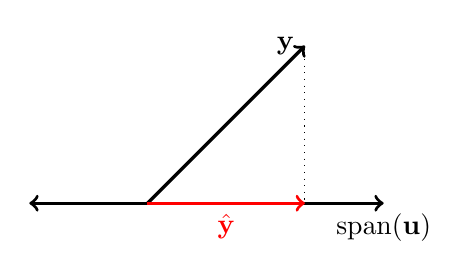
\begin{tikzpicture}
			\draw[very thick, <->](-1.5,0)--(3,0)node[below]{$\text{span}(\mathbf{u})$};
			\draw[very thick, ->](0,0)--(2,2)node[left]{$\mathbf{y}$};
			\draw[dotted](2,2)--(2,0);
			\draw[red,very thick,->](0,0)--(2,0)node[midway,below]{\color{red}$\hat{\mathbf{y}}$};
			\end{tikzpicture}
		\end{center}
		
		\item\underline{\smash{Aside}}.
		This idea extends to vectors that don't span the $x$-axis (it's just a bit easier to draw). Similarly, we can think
		about projections in an analagous way for multiple dimensions (although it is much harder to draw and much harder to
		picture mentally). Indeed, higher dimensionality is important--the fitted values from OLS, for example, are the projection
		of $\mathbf{y}$ onto the column space of the data matrix $\mathcal{X}$. Luckily, we have theorems to help us handle more dimensions.
		
	\end{enumerate}

\item\textbf{Orthogonality}
	%%%%%%%%%
	%LAY 6.1%
	%%%%%%%%%
	\begin{enumerate}
	\item\underline{\smash{Definition}}.
		Let $\mathbf{u}$ and $\mathbf{v}$ be vectors in $\mathbb{R}^n$. Then the \textbf{inner product} of the vectors is
		a scalar given by $\mathbf{u}^T\mathbf{v}$ or $\mathbf{u}\cdot\mathbf{v}$.
			\[\mathbf{u}^T\mathbf{v}=\begin{bmatrix}u_1&u_2&\dots&u_n\end{bmatrix}\begin{bmatrix}v_1\\v_2\\\dots\\v_n\end{bmatrix}
			=u_1v_1+u_2v_2+\dots+u_nv_n\]
		This is also known as the \textbf{dot product}.

	\item\underline{\smash{Aside}}.
		Note that we can write our usual notion of length, the Euclidian norm, in terms of inner product:
			\[||\mathbf{x}||_2=\sqrt{\mathbf{x}^T\mathbf{x}}=\left(\sum_{i=1}^nx_i^2\right)^{\frac{1}{2}}\]

	\item\underline{\smash{Definition}}.
		Two vectors $\mathbf{u}$ and $\mathbf{v}$ in $\mathbb{R}^n$ are orthogonal if and only if
		$\mathbf{u}^T\mathbf{v}=0$.

	\item\underline{\smash{Theorem}} (Lay THM 6.2).
		Two vectors $\mathbf{u}$ and $\mathbf{v}$ in $\mathbb{R}^n$ are orthogonal if and only if
			\[||\mathbf{u}+\mathbf{v}||^2 = ||\mathbf{u}||^2+||\mathbf{v}||^2\]
		This is the linear algebra version of the Pythagorean theorem.
	
	\item\underline{\smash{Aside}}.
		We can work through some of the algebra to show that this must be true if we're using the Euclidean norm. Note
		that $\mathbf{x}^T\mathbf{y}=\mathbf{y}^T\mathbf{x}=0$ if $\mathbf{x}$ and $\mathbf{y}$ are orthogonal:
		\begin{align*}
			||\mathbf{x}+\mathbf{y}||^2 & = (\mathbf{x}+\mathbf{y})^T(\mathbf{x}+\mathbf{y}) \\
			& = \mathbf{x}^T\mathbf{x}+\mathbf{y}^T\mathbf{x}+\mathbf{x}^T\mathbf{y}+\mathbf{y}^T\mathbf{y} \\
			& = ||\mathbf{x}||^2 + 0 + 0 +||+\mathbf{y}||^2 \\
			||\mathbf{x}+\mathbf{y}||^2 & = ||\mathbf{x}||^2 + ||\mathbf{y}||^2
		\end{align*}
		Now, the same steps can be used to show that $||\mathbf{x}-\mathbf{y}||^2=||\mathbf{x}||^2+||\mathbf{y}||^2$. This
		implies that $||\mathbf{x}+\mathbf{y}||^2=||\mathbf{x}-\mathbf{y}||^2$, or that $\mathbf{x}$ is equidistant
		to $\mathbf{y}$ and $-\mathbf{y}$. Graphically:
		\begin{center}
			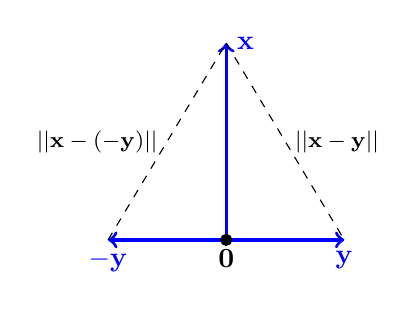
\begin{tikzpicture}
				\draw[very thick, color = blue,->] (0,0) -- (0,2.5)node[right]{$\mathbf{x}$};
				\draw[very thick, color = blue, <->] (-1.5,0)node[below]{$-\mathbf{y}$} -- (1.5, 0)node[below]{$\mathbf{y}$};
				\filldraw[black]circle(2pt)node[below]{$\mathbf{0}$};
				\draw[dashed](-1.5,0) -- (0,2.5)node[midway, left]{\footnotesize $||\mathbf{x}-(-\mathbf{y})||$};
				\draw[dashed](0,2.5) -- (1.5,0)node[midway, right]{\footnotesize$||\mathbf{x}-\mathbf{y}||$};;
			\end{tikzpicture}
		\end{center}
		In other words, orthogonal vectors are perpendicular to each other.
		
		\item\underline{\smash{Definition}}.
			Nonempty ``sets" $V,W \subset \mathbb{R}^n$ are orthogonal if and only if given any $\mathbf{v} \in V$, $\mathbf{w} \in W$ 
			\[ \mathbf{v}^T \mathbf{w} = 0 \]
			\textbf{Remark} The collection of vectors is not necessarily a vector space. 
			
		\item\underline{\smash{Theorem}}. 
		If $V,W \subset \mathbb{R}^n$ are orthogonal, then
			\[ V \cap W = \emptyset \ \vee \ V \cap W =\{\mathbf{0}\}\ \]
		
		\item\underline{\smash{Definition}}.
			Let $V$ be a subset of $\mathbb{R}^n$. The orthogonal complement of $V$, denoted by $V^\perp$, is the set of all vectors $\mathbf{w} \in \mathbb{R}^n$ that are orthogonal to the set $V$.
		
		\item\underline{\smash{Aside}}.
			\begin{enumerate}
				\item $V^\perp$ is a subspace of $\mathbb{R}^n$. 
				\item $\text{span}(V) = (V^\perp)^\perp$
			\end{enumerate}

		\item\underline{\smash{Theorem}} (Lay THM 6.3).
			Let $\mathcal{A}$ be a $m\times n$ matrix. The orthogonal complement of the row space of $\mathcal{A}$ is the null space of $\mathcal{A}$, and the orthogonal
			complement of the column space of $\mathcal{A}$ is the null space of $\mathcal{A}^T$:
				\[(\text{Col}(\mathcal{A}))^\perp=\text{Nul}(\mathcal{A}^T)\quad\text{and}\quad(\text{Row}(\mathcal{A}))^\perp = \text{Nul}(\mathcal{A})\]
			\begin{proof}
				\begin{align*}
					S &:= \{\mathbf{a}_1, \cdots, \mathbf{a}_n \} \subset \mathbb{R}^m  \\
					S^{\perp} &= \{\mathbf{w} \in \mathbb{R}^m : \mathbf{a}_i^T \mathbf{w} = 0 \ \mbox{ for all } \ i=1, \cdots, n \} \\
						&= \{\mathbf{w} \in \mathbb{R}^m : \mathcal{A}^T \mathbf{w} = \mathbf{0}_n \ \mbox{ for all } \ i=1, \cdots, n \} \\ 
					\text{Nul}(\mathcal{A}^T) &= \{ \mathbf{u} \in \mathbb{R}^m  \ : \ \mathcal{A}^T \mathbf{u} = \mathbf{0}_n  \} \\ 
						& = S^\perp  = \text{span}(S)^\perp = \text{Col}(\mathcal{A})^\perp
				\end{align*}
			\end{proof}
			
			\item\underline{\smash{Definition}}.
		A set of vectors $\{\mathbf{x}_1,\dots,\mathbf{x}_k\}$ in $\mathbb{R}^n$ is an \textbf{orthogonal set} if each pair of distinct
		vectors from the set are orthogonal. An \text{orthogonal basis} for a subspace $W\subset\mathbb{R}^n$ is a basis for $W$
		that is also an orthogonal set.
		
		\item\underline{\smash{Theorem}} (Lay THM 6.8).
		Let $W$ be a subspace of $\mathbb{R}^n$.
		Then each $\mathbf{y}\in\mathbb{R}^n$ can be written uniquely in the form
		\[\mathbf{y}=\hat{\mathbf{y}}+\hat{\mathbf{u}}\]
		where $\hat{\mathbf{y}}$ is in $W$ and $\hat{\mathbf{u}}\in W^{\perp}$. If $\{\mathbf{x}_1,\dots,\mathbf{x}_k\}$ is a
		basis of $W$, then
		\[\hat{\mathbf{y}}=\frac{\mathbf{y}'\mathbf{x}_1}{\mathbf{x}_1'\mathbf{x}_1}\mathbf{x}_1
		+\dots + \frac{\mathbf{y}'\mathbf{x}_k}{\mathbf{x}_k'\mathbf{x}_k}\mathbf{x}_k\]
		and $\hat{\mathbf{u}}=\mathbf{y}-\hat{\mathbf{y}}$. Here, $\hat{\mathbf{y}}$ is the orthogonal projection of $\mathbf{y}$
		onto $W$. This is known as the orthogonal decomposition theorem.
		
		\item\underline{\smash{Aside}}.
		To quick points are in order. First, this gives us a tool to understand how we can project $\mathbf{y}$ onto a higher-dimensional
		space than line spanned by a single vector. Second,
		note that the theorem states that any orthogonal basis can be used; it is the projection itself (not the basis) that is unique. Scale
		any vector in the basis (or analogously, any column in the data matrix $\mathcal{X}$) and it does not change the fitted values.
		
		\item\underline{\smash{Theorem}} (Lay THM 6.9).
		Let $W$ be a subspace of $\mathbb{R}^n$, let $\mathbf{y}\in\mathbb{R}^n$, and let
		$\hat{\mathbf{y}}$ be the orthogonal projection of $\mathbf{y}$ onto $W$. Then $\hat{\mathbf{y}}$ is the point in $W$
		closest to $\mathbf{y}$:
		\[||\mathbf{y}-\hat{\mathbf{y}}||<||\mathbf{y}-\mathbf{v}|| \ \text{for all} \ \mathbf{v}\in W \ni \mathbf{v}\neq\hat{\mathbf{y}}\]
		
		\begin{proof}
		\begin{align*}
		&||\mathbf{y}-\mathbf{v}|| = ||(\mathbf{y} - \hat{\mathbf{y}}) + (\hat{\mathbf{y}}-\mathbf{v})||
		&\text{(adding $\mathbf{0}$)}
		\intertext{Note that $\hat{\mathbf{y}}-\mathbf{v}\in W$ (both vectors ``live" in $W$, so their difference
			does as well. Further, note $\mathbf{y}-\hat{\mathbf{y}}\in W^{\perp}$ (by definition of orthogonal projection).
			Thus:}
		&||\mathbf{y}-\mathbf{v}||^2 =  ||\mathbf{y} - \hat{\mathbf{y}}||^2 + ||\hat{\mathbf{y}}-\mathbf{v}||^2
		&\text{(by the Pythaogrean Theorem)}\\[5pt]
		& ||\hat{\mathbf{y}}-\mathbf{v}||>0
		&(\mathbf{v}\neq\hat{\mathbf{y}}\text{ and by def. of a norm}) \\
		&\implies ||\mathbf{y}-\mathbf{v}||^2 > ||\mathbf{y} - \hat{\mathbf{y}}||^2
		&\text{(by $||\hat{\mathbf{y}}-\mathbf{v}||>0$)}	\\
		&\implies ||\mathbf{y}-\mathbf{v}|| > ||\mathbf{y} - \hat{\mathbf{y}}||
		&\text{(by non-negativity of norms)}
		\end{align*}
		\end{proof}
	\end{enumerate}



\item\textbf{OLS as a Projection}
	\begin{enumerate}
	\item\underline{\smash{Aside}}.
		Suppose We have large-dimensional problem $\mathcal{X}\mathbf{b} = \mathbf{y}$ (where $\mathcal{X}$ is $n\times k$,
		$\mathbf{b}$ is $k \times 1$, and $\mathbf{y}$ is $n \times 1$) that has no solution. Indeed, we
		frequently (i.e., ALWAYS as economists) have an inconsistent system. Thanks to the idea of orthogonal projections,
		however, we still have a solution concept.

	\item\underline{\smash{Definition}}.
		If $\mathcal{X}$ is a $n\times k$ matrix and $\mathbf{y}\in\mathbb{R}^n$, a \textbf{least-squares solution} of $\mathcal{X}\mathbf{b}=\mathbf{y}$
		is a $\widehat{\boldsymbol{\beta}}\in\mathbb{R}^k$ such that
		\[||\mathbf{y}-\mathcal{X}\widehat{\boldsymbol{\beta}}||\leq ||\mathbf{y}-\mathcal{X}\mathbf{b}|| \ \text{for all} \ \mathbf{b}\in\mathbb{R}^k\]
	
	\item\underline{\smash{Aside}}.
		Note that no matter what, the answer we pick is going to ``live" in the column space of $X$, $\text{Col}(\mathbf{X})$. Thus, we're
		trying to find the point in $\text{Col}(\mathcal{X})$ closest to $\mathbf{y}$. To do this, we'll use our best approximation theorem,
		which tells us that the closest point is the orthogonal projection. $\hat{\mathbf{y}}\in\text{Col}(\mathcal{X})$, so a solution
		to the system $\mathcal{X}\widehat{\boldsymbol{\beta}}=\hat{\mathbf{y}}$ \emph{will} exist.

	\item\underline{\smash{Theorem}} (Lay THM 6.14).
		Let $\mathcal{X}$ be a $n\times k$ matrix. The following statements are logically equivalent:
		\begin{enumerate}
		\item The equation $\mathcal{X}\mathbf{b}=\mathbf{y}$ has a unique least-squares solution for each $\mathbf{y}\in\mathbb{R}^n$
		\item the columns of $\mathcal{X}$ are linearly independent
		\item the matrix $\mathcal{X}^T\mathcal{X}$ is invertible
		\end{enumerate}
		When these statements are true, the least-squares solution $\hat{\boldsymbol{\beta}}$ is given by
			\[\widehat{\boldsymbol{\beta}}=(\mathcal{X}^T\mathcal{X})^{-1}\mathcal{X}^T\mathbf{y}\]
		\begin{proof}
		\begin{align*}
			\mathbf{0}_k & = \mathcal{X}^T(\mathbf{y}-\hat{\mathbf{y}})
					&\text{(by def. of orthogonal)}\\[5pt]
			\mathbf{0}_k & = \mathcal{X}^T(\mathbf{y}-\mathcal{X}\widehat{\boldsymbol{\beta}})
					&\text{(plugging in for $\hat{\mathbf{y}}$)}\\[5pt]
			\mathbf{0}_k & = \mathcal{X}^T\mathbf{y} - \mathcal{X}^T\mathcal{X}\widehat{\boldsymbol{\beta}}
					&\text{(distributing)}\\[5pt]
			\widehat{\boldsymbol{\beta}}& = (\mathcal{X}^T\mathcal{X})^{-1}\mathcal{X}^T\mathbf{y}
					&\text{(solving for $\widehat{\boldsymbol{\beta}}$)}
		\end{align*}
		\end{proof}
	
	
	%%%%%%%%%%
	%Ruud 2.4%
	%%%%%%%%%%
	\item\underline{\smash{Definition}}.
		Let $\mathcal{X}$ be a $n\times k$ matrix of full rank and let $\mathbf{y}\in\mathbb{R}^n$. Then the matrix
			\[\mathcal{P}_{\mathcal{X}} = \mathcal{X}(\mathcal{X}^T\mathcal{X})^{-1}\mathcal{X}^T\]
		is the \textbf{projection matrix} that projects $\mathbf{y}$ onto $\text{Col}(\mathcal{X})$.

	\item\underline{\smash{Theorem}} Let $\mathcal{P}_{\mathcal{X}}$ be the projection matrix where $\mathcal{P}_{\mathcal{X}}=\mathcal{X}(\mathcal{X}^T\mathcal{X})^{-1}\mathcal{X}^T$. Then $\mathcal{P}_{\mathcal{X}}$ is
		\begin{enumerate}
		\item Symmetric
		\item Idempotent
		\item Positive Semidefinite
		\end{enumerate}

	\item\underline{\smash{Definition}}.
		Let $\mathcal{P}_{\mathcal{X}}$ be the projection matrix associated with the columnn space of a $n\times k$ matrix $\mathcal{X}$. Then
		the \textbf{annihilator matrix} is defined as 
			\[\mathcal{M}_{\mathcal{X}} = I_n - \mathcal{P}_{\mathcal{X}}\]
		$\mathcal{M}_{\mathcal{X}}$ projects values of $\mathbf{y}\in\mathbb{R}^n$ onto Col$(\mathcal{X})^{\perp}$.  
		
		\textbf{Remark} Given $\mathbf{y} = \mathcal{X} \boldsymbol{\beta} + \mathbf{u}$, 
		\begin{enumerate}
			\item $\mathcal{M}_{\mathcal{X}}$ is symmetric, idempotent, and positive semidefinite. 
			\item $\mathcal{M}_{\mathcal{X}} \mathcal{X}=\mathbf{0}_n$
			\item $\hat{\mathbf{u}}=\mathcal{M}_{\mathcal{X}} \mathbf{y} = \mathcal{M}_{\mathcal{X}} \mathbf{u}$ and $\hat{\mathbf{u}}^T \hat{\mathbf{u}} = \mathbf{u}^T \mathcal{M}_{\mathcal{X}} \mathbf{u}$
			\item $\hat{\mathbf{u}} \in \text{Nul}(\mathcal{X}^T)$ and $\mathcal{X}^T \hat{\mathbf{u}} = \mathbf{0}$ \hfill ($n-k$ degrees of freedom) 
			\item $\text{rank}(\mathcal{M}_{\mathcal{X}}) = \text{tr}(\mathcal{M}_{\mathcal{X}}) = n-k$
		\end{enumerate}

	\item\underline{\smash{Aside}}.
		Depending on the presentation of OLS, the projection and annihilator matrices are important tools
		in developing the theory behind econometrics. Even if we focus on a more statistics-motivated
		approach to OLS, it is valuable to understand these matrices and what they do.
	\end{enumerate}

%%%%%%%%%%%
%WIKIPEDIA%
%%%%%%%%%%%
\item\textbf{Matrix Differentiation}
	\begin{enumerate}
	\item\underline{\smash{Aside}}.
		We won't get into the details, but it is occasionally helpful to employ differentiation at a
		matrix level; for example, we can derive an estimator $\widehat{\boldsymbol{\beta}}$ for the regression equation
		$y=X\beta+\varepsilon$ by minimizing $\varepsilon'\varepsilon$ via matrix differentiation. Here
		are a few of the formulas you'll likely run across:
		\begin{enumerate}
		\item Vector-by-Vector $y \in \mathbb{R}$ and $\mathbf{x} \in \mathbb{R}^n$
			\begin{enumerate}
			\item In general:
				\[\frac{\partial y}{\partial\mathbf{x}}=
				\begin{bmatrix}
				\frac{\partial y}{\partial x_1} \\[5pt]
				\frac{\partial y}{\partial x_2} \\
				\vdots \\ 
				\frac{\partial y}{\partial x_n} \\
				\end{bmatrix}  \hspace{5mm} \text{and} \hspace{5mm} 
				\frac{\partial y}{\partial\mathbf{x}^T}=
				\begin{bmatrix}
				\frac{\partial y}{\partial x_1} &
				\frac{\partial y}{\partial x_2} &
				\cdots &
				\frac{\partial y}{\partial x_n}
				\end{bmatrix}\] 
			\item For a vector of constants $a \in \mathbb{R}$:
				\[\frac{\partial a}{\partial \mathbf{x}}=\mathbf{0}_n\]
			\item For a derivative of a vector with respect to itself:
				\[\frac{\partial\mathbf{x}}{\partial\mathbf{x}}=I_n\]
			\end{enumerate}
		\item Matrix-by-Vector
			\begin{enumerate}
			\item Linear form:
				\begin{align*}
				\frac{\partial \mathcal{A}\mathbf{x}}{\partial\mathbf{x}^T}&=\mathcal{A} 
						&\text{(post-multiplied by $\mathbf{x}$)}\\
				\end{align*}
			\item Quadratic form:
				\begin{align*}
				\frac{\partial\mathbf{x}^T\mathcal{A}\mathbf{x}}{\partial\mathbf{x}^T}&=\mathbf{x}^T (\mathcal{A} + \mathcal{A}^T) 
						&\text{(if $\mathcal{A}$ is not symmetric)}\\[5pt]
				\frac{\partial\mathbf{x}^T \mathcal{A}\mathbf{x}}{\partial\mathbf{x}^T}&=2\mathbf{x}^T\mathcal{A}
						&\text{(if $\mathcal{A}$ is symmetric)}
				\end{align*}
			\end{enumerate}
		\end{enumerate}
	
	\item\underline{\smash{Example}}. Ordinary Least Square
	\[ \hat{\boldsymbol{\beta}} \in arg \min_{b \in \mathbb{R}^k} S(\mathbf{b}) \hspace{5mm} \text{where} \hspace{5mm} S(\mathbf{b}) = (\mathbf{y}-\mathcal{X}\mathbf{b})^T (\mathbf{y}-\mathcal{X}\mathbf{b}) \]
	
	\begin{align*}
		\frac{\partial S(\hat{\boldsymbol{\beta}})}{\partial \mathbf{b}^T} &= \mathbf{0} \\[5pt]
		2\hat{\boldsymbol{\beta}}^T (\mathcal{X}^T \mathcal{X}) - 2 \mathbf{y}^T \mathcal{X} &= 0 \\[5pt]
		(\mathcal{X}^T \mathcal{X}) \hat{\boldsymbol{\beta}} - \mathcal{X}^T \mathbf{y} &= 0 \\[5pt]
		\hat{\boldsymbol{\beta}} &= (\mathcal{X}^T \mathcal{X})^{-1} \mathcal{X}^T \mathbf{y} 
	\end{align*}
	
	\end{enumerate}

\newpage

\item\textbf{Appendix 1: Determinant}
	\begin{enumerate}
		\item $3 \times 3$ Matrix: $\mathcal{A}=\begin{bmatrix}
		a_{11} & a_{12} & a_{13} \\
		a_{21} & a_{22} & a_{23} \\
		a_{31} & a_{32} & a_{33}
		\end{bmatrix}$\\
		
		First method, multiply three elements diagonally to the right and sum; multiply three
		elements diagonally to the left and subtract. Visually, (solid = positive, dashed = negative):
		\begin{center}
			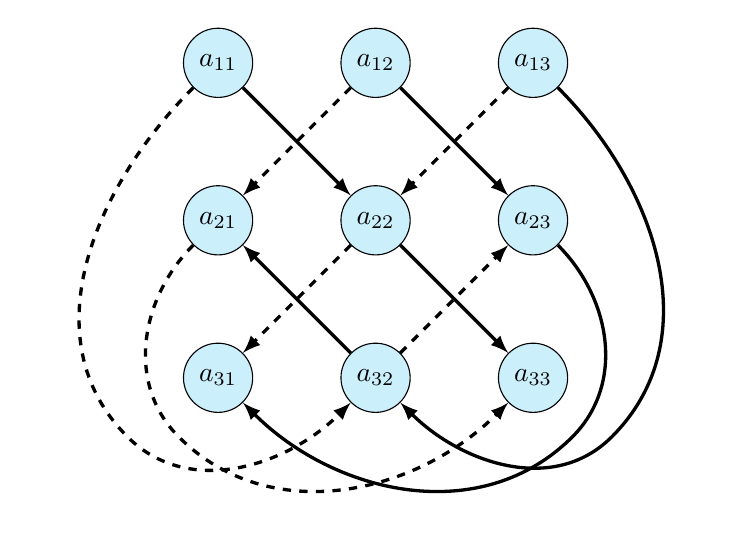
\begin{tikzpicture}[auto,node distance=2cm, >=latex]
			\tikzstyle{every state}=[fill=cyan!20]
			%First Row
			\node[state](a11){$a_{11}$};
			\node[state](a12)[right of = a11]{$a_{12}$};
			\node[state](a13)[right of = a12]{$a_{13}$};
			%Second Row
			\node[state](a21)[below of = a11]{$a_{21}$};
			\node[state](a22)[right of = a21]{$a_{22}$};
			\node[state](a23)[right of = a22]{$a_{23}$};
			%Third Row
			\node[state](a31)[below of = a21]{$a_{31}$};
			\node[state](a32)[right of = a31]{$a_{32}$};
			\node[state](a33)[right of = a32]{$a_{33}$};
			%Arrows Positive
			\draw[very thick, ->](a11)--(a22);
			\draw[very thick, ->](a22)--(a33);
			\draw[very thick, ->](a12)--(a23);
			\draw[very thick, ->](a23) to [out=-45,in=45] ($(a33)+(.5,-0.75)$) to [out=-135, in=-45 ] (a31);
			\draw[very thick, ->](a13) to [out=-45,in=45] ($(a23)+(1,-2.75)$) to [out=-135, in=-45 ] (a32);
			\draw[very thick, ->](a32)--(a21);
			%Arrows Negative
			\draw[very thick, dashed, ->](a13)--(a22);
			\draw[very thick, dashed, ->](a22)--(a31);
			\draw[very thick, dashed, ->](a12)--(a21);
			\draw[very thick, dashed, ->](a21) to [out=-135, in=135] ($(a31)+(-.5,-0.75)$)
			to [out=-45, in=-135 ] (a33);
			\draw[very thick, dashed, ->](a11) to [out=-135,in=135] ($(a21)+(-1.15,-2.75)$)
			to [out=-45, in=-135 ] (a32);
			\draw[very thick, dashed, ->](a32)--(a23);
			\end{tikzpicture}
		\end{center}
		$|\mathcal{A}|=a_{11}a_{22}a_{33}+a_{12}a_{23}a_{31}+a_{13}a_{32}a_{21}
		-a_{13}a_{22}a_{31}-a_{12}a_{21}a_{33}-a_{11}a_{32}a_{23}$\\
		
		\item For matrices $3\times 3$ and larger, use the Laplace Expansion.
		\begin{enumerate}
			\item\underline{\smash{Definition}}.
			The determinant of the matrix that results from deleting rows and columns
			associated with element $a_{ij}$ is the \textbf{minor} $|M_{ij}|$.
			
			\item\underline{\smash{Example}}.
			Consider again the $3\times 3$ matrix $A$ (defined above).
			The minor associated with the element $a_{11}$ is $|M_{11}|=\begin{vmatrix} a_{22} & a_{23} \\ 
			a_{32} & a_{33}\end{vmatrix}$.
			Visually, this can be represented:
			
			\begin{center}
				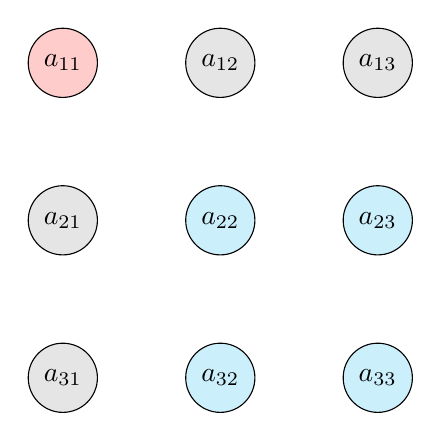
\begin{tikzpicture}[auto,node distance=2cm, >=latex]
				\tikzstyle{every state}=[fill=cyan!20]
				%First Row
				\node[state](a11)[fill = red!20]{$a_{11}$};
				\node[state](a12)[right of = a11, fill = gray!20]{$a_{12}$};
				\node[state](a13)[right of = a12, fill = gray!20]{$a_{13}$};
				%Second Row
				\node[state](a21)[below of = a11, fill = gray!20]{$a_{21}$};
				\node[state](a22)[right of = a21]{$a_{22}$};
				\node[state](a23)[right of = a22]{$a_{23}$};
				%Third Row
				\node[state](a31)[below of = a21, fill = gray!20]{$a_{31}$};
				\node[state](a32)[right of = a31]{$a_{32}$};
				\node[state](a33)[right of = a32]{$a_{33}$};
				\end{tikzpicture}
			\end{center}
			
			\vspace{5mm}
			
			The minor associated with $a_{22}$ is $|M_{22}|=\begin{vmatrix}	a_{11} & a_{13} \\ 
			a_{31} & a_{33}\end{vmatrix}$\\[5pt]
			\begin{center}
				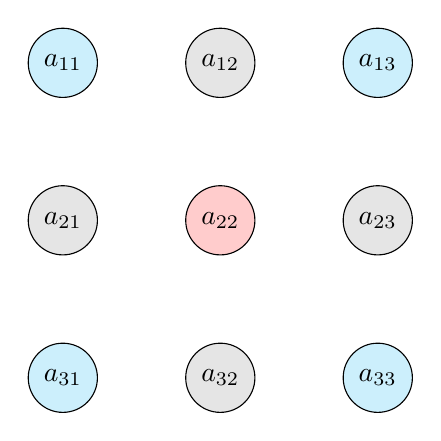
\begin{tikzpicture}[auto,node distance=2cm, >=latex]
				\tikzstyle{every state}=[fill=cyan!20]
				%First Row
				\node[state](a11){$a_{11}$};
				\node[state](a12)[right of = a11, fill = gray!20]{$a_{12}$};
				\node[state](a13)[right of = a12]{$a_{13}$};
				%Second Row
				\node[state](a21)[below of = a11, fill = gray!20]{$a_{21}$};
				\node[state](a22)[right of = a21, fill = red!20]{$a_{22}$};
				\node[state](a23)[right of = a22, fill = gray!20]{$a_{23}$};
				%Third Row
				\node[state](a31)[below of = a21]{$a_{31}$};
				\node[state](a32)[right of = a31, fill = gray!20]{$a_{32}$};
				\node[state](a33)[right of = a32]{$a_{33}$};
				\end{tikzpicture}
			\end{center}
			
			\vspace{5mm}
			
			\item\underline{\smash{Definition}}.
			The \textbf{cofactor} $|C_{ij}|$ is a minor modified by a prescribed algebraic sign that follows the convention:
			\[|C_{ij}|\equiv (-1)^{i+j}|M_{ij}|\]
			
			\item\underline{\smash{Definition}}. The determinant found by \textbf{Laplace Expansion} is the value found
			by ``expanding" along any row or column:
			\begin{align*}
			|A| & = \sum_{j=1}^na_{ij}|C_{ij}|	&\text{(expansion by the $i$th row)}\\
			|A| & = \sum_{i=1}^na_{ij}|C_{ij}|	&\text{(expansion by the $j$th column)}
			\end{align*}
			
			\item\underline{\smash{Example}}.
			Considering one again the $3\times 3$ matrix $C$ (defined above), performing the Laplace Expansion using the first row:
			\begin{align*}
			|\mathcal{A}| & = a_{11} |C_{11}| + a_{12} |C_{12}| + a_{13} |C_{13}| \\[5pt]
			|\mathcal{A}| & = (-1)^{1+1}\cdot  a_{11} \begin{vmatrix} a_{22} & a_{23} \\ a_{32} & a_{33}\end{vmatrix}
			+ (-1)^{1+2} \cdot a_{12} \begin{vmatrix} a_{21} & a_{31} \\ a_{23} & a_{33}\end{vmatrix}
			+ (-1)^{1+3} \cdot a_{13} \begin{vmatrix} a_{21} & a_{22} \\ a_{31} & a_{32}\end{vmatrix}
			\end{align*}
			
			\item\underline{\smash{Example}}.
			Consider the $3\times 3$ matrix $\mathcal{A}=\begin{bmatrix} -7 & 0 & 3 \\ 9 & 1 & 4 \\ 0 & 6 & 5 \end{bmatrix}$. Expanding
			along the top row:
			
			\begin{align*}
			|\mathcal{A}|& = (-7)\begin{vmatrix} 1 & 4 \\ 6 & 5\end{vmatrix}
			- (0)\begin{vmatrix} 9 & 4 \\ 0 & 5\end{vmatrix}
			+(3)\begin{vmatrix} 9 & 1 \\ 0 & 6\end{vmatrix} \\[5pt]
			&= -7(5-24) + 0 + 3(54-0) \\[5pt]
			&= 133 + 0 + 162 = 295 
			\end{align*}	
		\end{enumerate}
	\end{enumerate}

\newpage

\item\textbf{Appendix 2: Inverse}

	\begin{enumerate}
			\item\underline{\smash{Example}}.
		Suppose we have an invertible matrix
		\[\mathcal{A}=\begin{bmatrix}a_{11} & a_{12} & a_{13} \\ a_{21} & a_{22} & a_{23} \\ a_{31} & a_{32} & a_{33}\end{bmatrix}\]
		Then we could find the inverse of $A$ by performing row operations on the augmented matrix
		\[\left[\begin{array}{c |c} \mathcal{A} & I_3\end{array}\right]
		=\left[\begin{array}{c c c | c c c}
		a_{11}	&a_{12}	&a_{13}	&1	&0	&0	\\
		a_{21}	&a_{22}	&a_{23}	&0	&1	&0	\\
		a_{31}	&a_{32}	&a_{33}	&0	&0	&1
		\end{array}\right]\]
		until we arrived at a matrix of the form
		\[\left[\begin{array}{c|c}I_3 & \mathcal{A}^{-1}\end{array}\right]
		=\left[\begin{array}{c c c | c c c}
		1	&0	&0	&b_{11}	&b_{12}	&b_{13} \\
		0	&1	&0	&b_{21}	&b_{22}	&b_{23} \\
		0	&0	&1	&b_{31}	&b_{32}	&b_{33}
		\end{array}\right]\]
		
		
		
		%%%%%%%%%%%%
		%CHIANG 5.4%
		%%%%%%%%%%%%
		\item\underline{\smash{Theorem}} (CW SEC 5.4)
		If $\mathcal{A}$ is a $n\times n$ invertible matrix, the inverse may be found by using the determinant and cofactors
		of the matrix $\mathcal{A}$.
		\begin{enumerate}
			\item\underline{\smash{Definition}}.
			The \textbf{cofactor matrix} of $\mathcal{A}$ is a matrix defined by replacing the elements of $\mathcal{A}$ with their associated
			cofactors:
			\[C = \begin{bmatrix}	
			|C_{11}|	&|C_{12}|	 &\dots    &|C_{1n}|	\\
			|C_{21}|   &|C_{22}|	&\cdots &|C_{2n}		\\
			\vdots	   &\vdots		 &\ddots  &\vdots 	\\
			|C_{n1}|   & |C_{n2}|   & \dots   & |C_{nn}|	\end{bmatrix}\]
			\item\underline{\smash{Definition}}.
			The \textbf{adjoint} of $\mathcal{A}$ is the transpose of the cofactor matrix:
			\[\text{adj}(\mathcal{A})=C^T=\begin{bmatrix}	
			|C_{11}|	&|C_{21}|	 &\dots    &|C_{n1}|	\\
			|C_{12}|   &|C_{22}|	&\cdots &|C_{n2}		\\
			\vdots	   &\vdots		 &\ddots  &\vdots 	\\
			|C_{1n}|   & |C_{2n}|   & \dots   & |C_{nn}|	\end{bmatrix}\]
		\end{enumerate}
		The inverse of a $n\times n$ matrix $\mathcal{A}$ can be found via the formula:
		\[\mathcal{A}^{-1}=\frac{1}{|\mathcal{A}|}\text{adj}(\mathcal{A})\]
		
		\item\underline{\smash{Example}}.
		Consider the $3\times 3$ matrix $\mathcal{A}$:
		\[\mathcal{A} = \begin{bmatrix}	0	&1	&0	\\
		2	&1	&2	\\
		4	&0	&0
		\end{bmatrix}\]
		First, we can take the determinant to establish invertibility:
		\begin{align*}
		|\mathcal{A}| & = 0\begin{vmatrix}1 & 2 \\ 0 & 0\end{vmatrix} - 1\begin{vmatrix}2 & 2\\ 4 & 0\end{vmatrix}
		+0\begin{vmatrix}2 & 1 \\ 4 & 0\end{vmatrix}
		&\text{(expanding on 1st row)}\\[5pt]
		& = 0 -1(0-8) + 0 = 8
		&\text{(simplifying)}
		\intertext{Since $|\mathcal{A}|\neq 0$, we can inverst this matrix. Next, find the cofactor matrix $C_{\mathcal{A}}$:}
		C_{\mathcal{A}} & =\left[\begin{array}{r r r}
		\begin{vmatrix}1&2\\0&0\end{vmatrix}&-\begin{vmatrix}2&2\\4&0\end{vmatrix}&\begin{vmatrix}2&1\\4&0\end{vmatrix} \\[20pt]
		-\begin{vmatrix}1&0\\0&0\end{vmatrix}&\begin{vmatrix}0&0\\4&0\end{vmatrix}&-\begin{vmatrix}0&1\\4&0\end{vmatrix} \\[20pt]
		\begin{vmatrix}1&0\\1&2\end{vmatrix}&-\begin{vmatrix}0&0\\2&2\end{vmatrix}&\begin{vmatrix}0&1\\2&1\end{vmatrix}
		\end{array}\right]
		&\text{(the cofactor matrix)}\\[5pt]
		C_{\mathcal{A}} & = \begin{bmatrix}0&8&-4\\0&0&4\\2&0&-2\end{bmatrix}
		&\text{(simplifying)}
		\intertext{Recall that the adjoint of $A$ is the transpose of $C_{\mathcal{A}}$:}
		\text{adj}(\mathcal{A}) & = C_{\mathcal{A}}^T
		&\text{(by def. of the adjoint)}\\[5pt]
		\text{adj}(\mathcal{A}) & = \begin{bmatrix}0&0&2\\8&0&0\\-4&4&-2\end{bmatrix}
		&\text{(the adjoint matrix)}
		\intertext{Finally, we can calculate the inverse of $\mathcal{A}$:}
		\mathcal{A}^{-1} & = \frac{1}{|\mathcal{A}|}\text{adj}(A)
		&\text{(the inverse formula)}\\[5pt]
		&=\frac{1}{8}\begin{bmatrix}0&0&2\\8&0&0\\-4&4&-2\end{bmatrix}
		&\text{(plugging in values)}\\[5pt]
		\mathcal{A}^{-1} & = \begin{bmatrix}0&0&1/4\\1&0&0\\-1/2&1/2&-1/4\end{bmatrix}
		&\text{(the inverse)}
		\end{align*}
	\end{enumerate}

\newpage

\item\textbf{Appendix 3: Cramer's Rule}

\begin{enumerate}
		\item\underline{\smash{Example}} (CW SEC 5.6).
	Consider a two-commodity, linear market model. For the first market:
	\begin{align*}
	Q_{d1} & = a_0 + a_1P_1 + a_2P_2
	&\text{(demand 1)}\\[5pt]
	Q_{s1} & = b_0 + b_1P_1 +b_2P_2
	&\text{(supply 1)}\\[5pt]
	0 & = Q_{d1} - Q_{s1}
	&\text{(S = D)}
	\intertext{For the second:}
	Q_{d2} & = \alpha_0 + \alpha_1P_1 + \alpha_2P_2
	&\text{(demand 2)}\\[5pt]
	Q_{s2} & = \beta_0 + \beta_1P_1 +\beta_2P_2
	&\text{(supply 2)} \\[5pt]
	0&=Q_{d2} - Q_{s2}
	&\text{(S = D)}
	\intertext{This reduces into a two-equation, two-unknown system:}
	0&=(a_0\!-\!b_0)+(a_1\!-\!b_1)P_1 + (a_2\!-\!b_2)P_2
	&\text{(for market 1)}\\[5pt]
	0&=(\alpha_0\!-\!\beta_0)+(\alpha_1\!-\!\beta_1)P_1 + (\alpha_2\!-\!\beta_2)P_2
	&\text{(for market 2)}
	\intertext{Rewriting for expediency, defining $c_i=a_i-b_i$ (and analogously for greek letters):}
	c_1P_1+c_2P_2 & =-c_0
	&\text{(market 1)}\\[5pt]
	\gamma_1 P_1 + \gamma_2 P_2 & = -\gamma_0
	&\text{(market 2)}
	\intertext{Rewriting in matrix notation:}
	\begin{bmatrix} c_1 & c_2 \\ \gamma_1 & \gamma _2 \end{bmatrix}
	\begin{bmatrix} P_1 \\ P_2\end{bmatrix}
	& = \begin{bmatrix} -c_0 \\ -\gamma_0\end{bmatrix}
	&\text{(the linear system)}
	\intertext{Solving for $P_1^*$ (the market clearing price for good 1):}
	P_1^*& = \frac{\begin{vmatrix}-c_0 & c_2 \\ -\gamma_0 & \gamma_2 \end{vmatrix}}
	{\begin{vmatrix} c_1 & c_2 \\ \gamma_1 & \gamma _2 \end{vmatrix}}
	=\frac{c_2\gamma_0-c_0\gamma_2}{c_1\gamma_2-c_2\gamma_1}
	&\text{(by Cramer's Rule)}
	\intertext{Solving for $P_2^*$ (the market clearing price for good 2):}
	P_2^*& = \frac{\begin{vmatrix}c_1 & -c_0 \\ \gamma_1 & -\gamma_0 \end{vmatrix}}
	{\begin{vmatrix} c_1 & c_2 \\ \gamma_1 & \gamma _2 \end{vmatrix}}
	=\frac{c_0\gamma_1-c_1\gamma_0}{c_1\gamma_2-c_2\gamma_1}
	&\text{(by Cramer's Rule)}
	\end{align*}
\end{enumerate}

\end{enumerate}
\end{document}